\documentclass[12pt,a4paper]{report}
\usepackage[utf8]{inputenc}
\usepackage[T1]{fontenc}
\usepackage{amsmath,amsfonts,amssymb,setspace,graphicx,array,fancyhdr,geometry,booktabs,float,longtable,tabularx}
\usepackage[table]{xcolor}
\usepackage{tikz,pgfplots,listings,url,hyperref}
\usetikzlibrary{arrows.meta,positioning,shapes.geometric}
\pgfplotsset{compat=1.18}
\geometry{a4paper,left=1.25in,right=.75in,top=.75in,bottom=.75in}
\setlength{\headheight}{15pt}
\setlength{\emergencystretch}{3em}
\hypersetup{hidelinks,pdftitle={Learning Sustained Contacts from RSSI, Angular Measurements, and Ranging: A Reproducible Simulation Study},pdfauthor={Arjun KV, Ayyan Anwar, Md Aasim Shaibani, Nabil Ahmad Khan}}
\urlstyle{same}
\graphicspath{{assets/logos/}{assets/screenshots/}}
\lstset{basicstyle=\ttfamily\footnotesize,breaklines=true,breakatwhitespace=false,columns=fullflexible,frame=single,keepspaces=true}
\linespread{1.4}
\newcommand{\projecttitle}{Learning Sustained Contacts from RSSI, Angular Measurements, and Ranging: A Reproducible Simulation Study}
\newcommand{\collegeheading}{\begin{center}{\LARGE\bfseries SAHYADRI}\par\vspace{5pt}{\Large\bfseries College of Engineering \& Management}\par\vspace{3pt}{\large Adyar, Mangaluru -- 575 007}\par\vspace{14pt}{\large\bfseries Department of Computer Science \& Engineering}\par\vspace{6pt}
\includegraphics[height=.85in]{sahyadri.png}\end{center}}
\begin{document}
\pagestyle{empty}
\begin{titlepage}
\begin{center}
{\large\bfseries VISVESVARAYA TECHNOLOGICAL UNIVERSITY}\par
{\large\bfseries ``JNANA SANGAMA'', BELAGAVI -- 590 018}\par
\vspace{6pt}
\includegraphics[height=.7in]{vtu.jpg}\par\vspace{6pt}
{\Large\bfseries PROJECT PHASE II REPORT}\par
\vspace{4pt}on\par\vspace{7pt}
{\large\bfseries ``\projecttitle''}\par
\vspace{8pt}
{\small Simulation-Based Study of Sustained Contacts Using RSSI, Angular Measurements, and Ranging}\par
\vspace{12pt}\textit{Submitted by}\par\vspace{8pt}
\begin{tabular}{lr}
\textbf{Arjun KV}&\textbf{4SF23CS032}\\
\textbf{Ayyan Anwar}&\textbf{4SF23CS042}\\
\textbf{Md Aasim Shaibani}&\textbf{4SF23CS103}\\
\textbf{Nabil Ahmad Khan}&\textbf{4SF23CS123}
\end{tabular}\par
\vspace{12pt}
\textit{In partial fulfillment of the requirements for the VII semester}\par
\textbf{BACHELOR OF ENGINEERING}\par in\par
\textbf{COMPUTER SCIENCE \& ENGINEERING}\par
\vspace{10pt}\textit{Under the Guidance of}\par
\textbf{Ms. Alakananda K}\par
{\small Assistant Professor, Department of CSE}\par
\vspace{8pt}
\includegraphics[height=.65in]{sahyadri.png}\par
\vspace{5pt}{\Large\bfseries SAHYADRI}\par
{\large\bfseries College of Engineering \& Management}\par
{\large An Autonomous Institution}\par
{\large MANGALURU}\par
\vspace{8pt}{\large\bfseries 2026 -- 27}
\end{center}
\end{titlepage}
\collegeheading
\begin{center}\vspace{8pt}{\Large\bfseries CERTIFICATE}\end{center}
\setstretch{1.5}
\noindent This is to certify that the Project Phase II work entitled \textbf{``\projecttitle''} has been carried out by \textbf{Arjun KV (4SF23CS032), Ayyan Anwar (4SF23CS042), Md Aasim Shaibani (4SF23CS103), and Nabil Ahmad Khan (4SF23CS123)}, bonafide students of Sahyadri College of Engineering and Management, under the guidance of \textbf{Ms. Alakananda K}, in partial fulfillment of the requirements for the VII semester of Bachelor of Engineering in Computer Science and Engineering of Visvesvaraya Technological University, Belagavi, during the academic year 2026--27.

\noindent The report documents the project architecture, implementation, and simulation-based experimental evaluation. Institutional endorsement and approval are recorded through the signatures below.
\vspace{.85in}
\setstretch{1.1}
\begin{center}\small
\begin{tabularx}{\textwidth}{>{\centering\arraybackslash}X >{\centering\arraybackslash}X >{\centering\arraybackslash}X}
\rule{.27\textwidth}{.4pt}&\rule{.27\textwidth}{.4pt}&\rule{.27\textwidth}{.4pt}\\[6pt]
\textbf{Project Guide}&\textbf{Project Coordinator}&\textbf{HOD}\\
Ms. Alakananda K&Dr. Poornima B V&Dr. Mustafa Basthikodi\\
Assistant Professor&Associate Professor&Professor \& Head\\
Dept. of CSE&Dept. of CSE&Dept. of CSE
\end{tabularx}\end{center}
\clearpage
\collegeheading
\begin{center}\vspace{8pt}{\Large\bfseries DECLARATION}\end{center}
\setstretch{1.5}
\noindent We hereby declare that the work embodied in this Project Phase II report entitled \textbf{``\projecttitle''} has been carried out by us at Sahyadri College of Engineering and Management, Mangaluru, under the supervision of \textbf{Ms. Alakananda K}, in partial fulfillment of the requirements for the VII semester of Bachelor of Engineering in Computer Science and Engineering.

\noindent This report has not been submitted to this or any other university for the award of another degree. The implementation, references, experimental assumptions, and limitations are identified in the report. The results are synthetic contact-reconstruction outcomes and do not constitute clinical or hospital hardware validation.
\vspace{.4in}
\begin{flushleft}
\textbf{Arjun KV (4SF23CS032)}\\[12pt]
\textbf{Ayyan Anwar (4SF23CS042)}\\[12pt]
\textbf{Md Aasim Shaibani (4SF23CS103)}\\[12pt]
\textbf{Nabil Ahmad Khan (4SF23CS123)}\\[12pt]
Dept. of CSE, SCEM, Mangaluru
\end{flushleft}
\clearpage
\pagestyle{plain}\pagenumbering{roman}
\chapter*{Abstract}\addcontentsline{toc}{chapter}{Abstract}
Reconstructing sustained person-to-person contacts from wireless telemetry requires reliable temporal decisions, not merely accurate individual distance estimates. We present a reproducible simulation study motivated by wearable contact monitoring in hospitals. Eight moving tags and four gateways occupy a two-room environment, and all 28 unordered pairs are evaluated each second. Seven observation configurations comprise received signal strength indicator (RSSI), RSSI with two or four angular receivers, RSSI with phase-based ranging (PBR), round-trip time (RTT), PBR with an RTT consistency gate, and ultra-wideband double-sided two-way ranging (UWB DS-TWR). Causal filtering and tracking produce 29 observable features without access to hidden geometry. Logistic regression, random forests, gradient-boosted trees, and Gaussian naive Bayes are fitted using disjoint training, probability-calibration, and validation recordings. Models and decision settings are frozen before 30 primary test recordings and 12 recordings with unseen motion are generated. Against equally validation-tuned geometric rules, selected models attain mean sustained-contact F1 scores of 0.445, 0.571, 0.704, 0.690, 0.561, 0.664, and 0.763, respectively. RSSI improves contact recovery but produces 464 false sessions across matched test conditions. UWB's incremental learned-versus-rule F1 difference is 0.034, with a pointwise seed-paired 95\% interval of -0.009 to 0.082. A learned Markov extension does not improve the selected classifiers. The results identify benefits and failure modes of learned contact reconstruction under explicit synthetic channel and scheduling assumptions. They do not establish hardware accuracy, clinical usefulness, battery life, or minimum deployment cost.

\noindent\textbf{Keywords:} contact reconstruction; BLE; RSSI; angle of arrival; phase-based ranging; RTT; UWB; probability calibration; reproducible simulation.
\chapter*{Acknowledgement}\addcontentsline{toc}{chapter}{Acknowledgement}
We express our sincere gratitude to our guide, Ms. Alakananda K, Assistant Professor, Department of Computer Science and Engineering, for her guidance and support throughout this project.

We thank Dr. Poornima B V and Dr. Deepti Rai, Project Coordinators, and Dr. Mustafa Basthikodi, Professor and Head of the Department of Computer Science and Engineering, for their encouragement and departmental support. We also thank Dr. S. S. Injaganeri, Principal, Sahyadri College of Engineering and Management.

We acknowledge the published research, technical documentation, and open-source software cited in this report. Their contributions support the sensing models, learning implementations, and reproducibility workflow. Finally, we thank our families and friends for their encouragement during the work.
\begin{flushright}\textbf{Arjun KV (4SF23CS032)}\\\textbf{Ayyan Anwar (4SF23CS042)}\\\textbf{Md Aasim Shaibani (4SF23CS103)}\\\textbf{Nabil Ahmad Khan (4SF23CS123)}\end{flushright}
\setstretch{1.4}
\renewcommand{\contentsname}{Table of Contents}
\tableofcontents\addcontentsline{toc}{chapter}{Table of Contents}
\listoffigures\addcontentsline{toc}{chapter}{List of Figures}
\listoftables\addcontentsline{toc}{chapter}{List of Tables}
\clearpage\pagestyle{fancy}\fancyhf{}
\lhead{\fontsize{10}{12}\selectfont Sustained Contact Reconstruction}
\rhead{\fontsize{10}{12}\selectfont Chapter \thechapter}
\lfoot{\fontsize{8}{10}\selectfont Department of Computer Science and Engineering, SCEM, Mangaluru}
\rfoot{\fontsize{10}{12}\selectfont Page \thepage}
\renewcommand{\headrulewidth}{.5pt}\renewcommand{\footrulewidth}{.5pt}
\setstretch{1.5}\pagenumbering{arabic}

\chapter{Introduction}

\section{Overview}
This research project is motivated by the difficulty of reconstructing interpersonal encounters from wireless evidence in a hospital setting. The original application combines simulated BLE observations, edge processing, identity-management experiments, and a dashboard. The final research contribution is a reproducible simulation of sustained-contact reconstruction using seven observation configurations and four trained classifier families.

This report presents the research study under the same title as the accompanying manuscript while retaining the supplied college chapter structure. The experimentally validated learning target is instantaneous geometric proximity, and the primary outcome is reconstructed sustained contact. Hospital use motivates the study; privacy mechanisms and the historical MDR-TB dashboard are companion prototype work rather than validated clinical outcomes. No probability in the main study is an infection probability, and the simulation does not establish a deployed privacy guarantee.

Digital contact records can supplement an investigation, but their usefulness depends on whether the sensing pipeline recovers actual encounters. A gateway observing two tags does not prove that the tags are within two metres. Even good individual ranges can fail to produce stable contact intervals when updates are missing or biased. The project therefore evaluates the entire observation-to-session chain rather than relying on a nominal sensor-accuracy claim.

The system is developed in generations. Earlier gateway co-observation results are retained as negative evidence. Angular localization, causal tracking, and phase/timing ranging were added in separately versioned experiments. The main learned study evaluates all unordered pairs before session detection, avoiding the limitation that a downstream scorer can only assess contacts that an earlier stage already found.

\section{Scope}
The completed work covers synthetic movement generation, radio-observation generation, causal measurement processing, robust localization, Kalman tracking, symmetric observable feature construction, classifier training, separate probability calibration, validation selection, temporal decoding, session matching, and reproducible reporting. Seven configurations include RSSI, RSSI with two or four angular receivers, PBR, RTT, PBR with an RTT consistency gate, and UWB double-sided two-way ranging.

The main environment contains eight moving tags, four anchors, one two-room floor plan, and 360 one-second frames per recording. Training, validation, calibration, primary testing, and unseen-motion testing use separate recording seeds. The study tests declared algorithms and parameter grids, not every possible learning or sensing technique.

The retained demonstration and historical privacy modules are described separately from the main learned experiment. Real BLE/UWB devices, antenna arrays, clinical participants, patient records, complete cryptographic deployment, wearable power measurements, hardware cost quotations, and hospital-wide field validation are outside the completed experimental scope. The public map is available to inference, while hidden true positions are used only for observation generation and reference construction.

\section{Motivation}
The first motivation is scientific: contact reconstruction must be tested against an independent reference. If the simulator directly turns geometric truth into displayed contacts, it demonstrates a scenario but does not evaluate wireless inference. The revised research generates radio observations and then reconstructs contacts without reading hidden geometry.

The second motivation is temporal reliability. One incorrect frame can split a sustained run; repeated small errors can also create a long false encounter. Frame probability quality, event recovery, interval coverage, and confirmation delay are therefore different concerns.

The third motivation is realistic comparison. Additional angles or ranges should be judged using the same movement and contact definitions. Learned methods should be compared with validation-tuned rules, so a gain is not merely the effect of adjusting a threshold that the baseline was denied.

The fourth motivation is affordability. Reusable hospital tags and infrastructure have acquisition and operating costs. The simulation can identify candidate sensing/accuracy tradeoffs, but choosing a minimum-cost system requires real quotations and measured capacity, energy, calibration, installation, and handling costs. Retaining UWB as a comparator is more informative than excluding it based on an unmeasured price assumption.

\chapter{Related Work}

\section{Healthcare-Associated TB Transmission and Infection Prevention}
The World Health Organization presents tuberculosis infection prevention and control through integrated administrative, environmental, and respiratory-protection measures \cite{ref17}. This project is motivated by the possible value of structured contact histories within that wider setting. It does not replace those measures or infer their effectiveness from radio data.

Proximity is a limited observational construct. It excludes ventilation, aerosol concentration, infectiousness, protective equipment, exposure dose, and biological susceptibility. A two-metre same-room event is the simulator's operational label, not a universal clinical transmission definition. No patients were recruited and no clinical outcomes were collected.

Consequently, this report avoids numerical claims about MDR-TB incidence reduction, infection probability, or clinical risk calibration. Such questions require independent epidemiological data and appropriate institutional approvals. The completed technical evaluation concerns whether synthetic geometric contacts can be recovered from uncertain measurements.

\section{BLE-Based Proximity Sensing}
Vanhems et al. used wearable proximity sensors to study interaction patterns in a hospital ward \cite{ref1}. Their work establishes a relevant application context but differs from our simulation in sensor technology, participants, sampling, and objectives. We do not reproduce that study or claim that our trajectories represent measured hospital routines. Leith and Farrell reported that BLE received signal strength is sensitive to handset orientation, body absorption, and the surrounding environment \cite{ref2}. This supports treating RSSI as uncertain evidence, not assuming that its inversion gives a dependable physical distance.

The present task separates instantaneous proximity from sustained contacts. A frame classifier can obtain useful discrimination while still producing long false sessions or breaking valid contacts into short segments. Conversely, a temporal decision can improve event recovery while extending predicted boundaries beyond the true interval. We therefore report event counts, contact F1, missed pair-time, false-session burden, duration error, and confirmation delay in addition to frame probability metrics.

Bluetooth Direction Finding obtains directional information through suitable radio procedures and antenna configurations \cite{ref3}. Our angular branch uses noisy two-dimensional bearings; it does not process IQ samples or simulate antenna arrays. Channel Sounding uses phase-based ranging and round-trip timing [4,5], but the specification does not prescribe a single distance-estimation algorithm \cite{ref4}. Our phase-slope and corrected-timing estimators are simplified algorithmic choices, not implementations of a complete Bluetooth controller or protocol stack.

Rathje and Landsiedel analyze bias and variance in double-sided two-way ranging and related TDoA extraction under multipath and non-line-of-sight conditions \cite{ref6}. Their analysis motivates explicit timing-error treatment; it does not supply measured parameters for the present simulator. We implement ideal DS-TWR intervals and assumed errors. UWB TDoA, anchor synchronization, real channel impulse responses, and firmware timestamping are outside the implemented scope.

\section{Wearable Contact Monitoring in Healthcare}
Vanhems et al. studied contact patterns in hospital wards with wearable proximity sensors \cite{ref1}. Their study establishes an application context, but its sensor technology, participants, time sampling, and aims differ from this simulation. The current project does not reproduce that field study or treat its designed motion patterns as measured hospital routines.

A wearable monitoring system must identify which tags interact and when, while handling missing observations, environmental error, and session boundaries. Device-level radio measurements become useful interpersonal evidence only after estimation and temporal interpretation. This distinction motivates the end-to-end event evaluation in the present work.

The final dataset includes deliberately brief encounters, near-boundary phases, doorway routes, and wall-separated proximity. These fixtures test particular failure modes rather than offering a representative census of hospital behavior.

\section{Edge Computing for Healthcare IoT}
Edge processing places computation near the acquisition point. In the original TypeScript pipeline, modules validate and normalize packets, remove duplicates, filter RSSI, create temporal pair evidence, and form sessions before downstream evaluation. This modular organization makes input/output dependencies inspectable.

The final research uses an additive offline simulation and learning workflow. Filtering, estimation, feature generation, and temporal decisions are algorithmically suitable for causal processing, but they have not been deployed on a hospital gateway. Desktop CPU time is not equivalent to gateway latency, radio procedure time, or wearable energy.

The design principle is to preserve useful contact evidence while reducing redundant representation. A system can compress a stream efficiently and still reconstruct the wrong contacts. Therefore no communication-reduction percentage is presented as proof of contact quality, and no unverified reduction value from the old report is transferred to the main study.

\section{Privacy-Preserving Digital Contact Tracing}
The historical source includes pseudonym generation, identifier-rotation schedules, an authorized identity registry, observation rewriting, and linkage/identity-inference experiments. These components distinguish direct identity exposure from behavioral linkability.

There are two implemented generator modes: keyed HMAC-SHA256 and a deterministic simulation-grade pseudo-random mode. The latter supports repeatable experiments but must not be called cryptographically secure. Security in the keyed mode depends on actual key secrecy, entropy, provisioning, and the surrounding deployment, none of which is established by the main v7 experiment.

Changing a broadcast identifier does not erase timing, receiver patterns, or movement continuity. These can remain linkable. The final v7 contact benchmark maintains synthetic stable tag identities for causal histories; it does not jointly evaluate rotating identifiers and its learned contact detector. This is an important integration limitation rather than a privacy result to be inferred from F1.

\section{Probabilistic Exposure-Risk Assessment}
Niculescu-Mizil and Caruana showed that classifier scores can exhibit model-dependent probability distortions and examined calibration approaches \cite{ref7}. Guo et al. likewise distinguish predictive performance from confidence calibration \cite{ref8}. These studies motivate assessing probability quality separately from thresholded contacts; they do not establish that the present probabilities are calibrated for hardware data. We use a sigmoid calibration map fitted to independent simulation recordings and report Brier score and ten-bin expected calibration error (ECE).

Classifiers are implemented with scikit-learn \cite{ref9}. Recording groups remain disjoint across partitions, following the principle that dependent observations should not be randomly split into nominally independent training and test examples \cite{ref10}. The histogram-gradient-boosting implementation is documented for the software version used here \cite{ref11}. We compare established model families under one frozen contact-reconstruction protocol. We do not infer that a family is generally superior from this small synthetic benchmark.

Three probability interpretations must be separated. The main models predict instantaneous synthetic same-room proximity. The original downstream scoring task concerns validity of surviving reconstructed records. A biological infection probability would concern a different clinical outcome. Neither of the first two becomes the third merely by using the term risk.

The original fixed-likelihood Bayesian scorer is also different from the learned Gaussian Bayes classifier and the learned Markov extension in v7. These methods use different targets, fitted quantities, and protocols. This report identifies those differences rather than pooling their outcomes into a model hierarchy.

\section{Research Gap}
The practical research gap is the mismatch between attractive individual sensing measurements and dependable sustained-contact recovery. A position or range can be reasonable on average while a temporal contact detector misses whole events, fragments runs, or generates persistent false sessions.

The project addresses this gap with matched observation budgets, independent geometric labels, all-pair evaluation, grouped partitions, separate calibration, frozen model selection, tuned deterministic controls, temporal extensions, feature ablations, and retained per-recording evidence. It examines both improvement and failure under explicit assumptions.

The contribution is the experimental framework and documented findings. The sensing principles, logistic regression, forests, boosting, and Gaussian Bayes are established methods; the report does not claim to invent them.

\chapter{Problem Formulation}

\section{Problem Description}
The primary environment is a 24 m by 20 m rectangle divided by a wall at x = 12 m. A doorway spans y = 9--11 m. Four public gateways are located at (2,2), (22,2), (22,18), and (2,18) m, with orientations 0, pi/2, pi, and -pi/2 radians. The two-receiver angular configuration upgrades gateways (2,2) and (22,18); the four-receiver configuration upgrades all four. Eight tags move over 360 one-second frames, yielding 28 unordered pairs and 10,080 pair-frames per motion recording.

Three motion families supply training, calibration, validation, and primary test recordings. Ward encounters randomize pair assignment, encounter location, onset, duration, and separation, with sustained approaches and brief encounters. Doorway rounds use continuous routes through the doorway and varying follower separations. Threshold encounters place close and far phases near the 2 m decision boundary. In the ward and threshold families, an always-close pair separated by the wall tests the importance of the same-room criterion. Tag assignments are shuffled so that pair identity cannot encode an encounter role.

The separately evaluated motion challenge gives each tag independent waypoints, movement speeds of 0.35--0.75 m/s, and pauses, with cross-room routes passing through the doorway. It changes the movement family while retaining the floor plan and radio assumptions. We call it unseen motion, not external hospital validation. The construction maintains continuous movement and verifies wall crossings and a maximum sampled step of 1.2 m.


\begin{figure}[htbp]
\centering
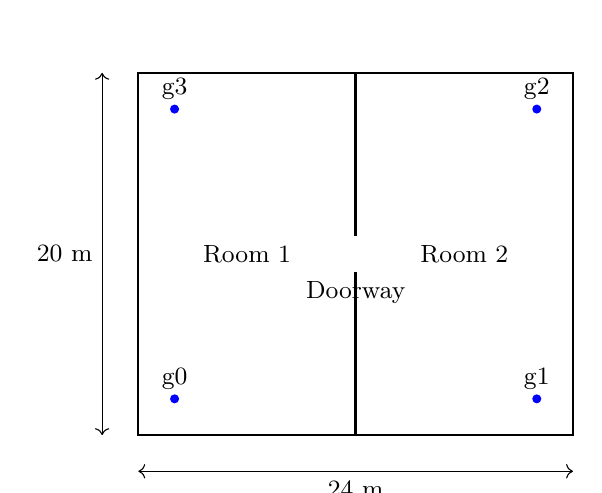
\begin{tikzpicture}[x=.23cm,y=.23cm, font=\small]
\draw[thick] (0,0) rectangle (24,20);
\draw[very thick] (12,0)--(12,9);\draw[very thick] (12,11)--(12,20);
\node at (6,10){Room 1};\node at (18,10){Room 2};
\node[below] at (12,9){Doorway};
\foreach \x/\y/\lab in {2/2/g0,22/2/g1,22/18/g2,2/18/g3}{\fill[blue] (\x,\y) circle (.25);\node[above] at (\x,\y){\lab};}
\draw[<->] (0,-2)--node[below]{24 m}(24,-2);\draw[<->] (-2,0)--node[left]{20 m}(-2,20);
\end{tikzpicture}
\caption{Public two-room geometry and anchor coordinates}\label{fig:floorplan}
\end{figure}


Let zi(t) be the hidden two-dimensional position of tag i at integer time t, and let r(z) identify its room. The instantaneous physical label for an unordered pair is

\begin{equation}
y_{ij}(t)=\mathbf{1}\{\lVert z_i(t)-z_j(t)\rVert_2\leq 2\,\mathrm{m}\}\,\mathbf{1}\{r(z_i(t))=r(z_j(t))\}
\label{eq:source1}
\end{equation}

A sustained reference session is a maximal consecutive run of positive samples with end time b and start time a satisfying b - a >= 30 s. Thus samples at t = 0,...,30 qualify, whereas 30 samples spanning t = 0,...,29 do not. This is sampled proximity, not a continuous-time check between samples. Short encounters are retained as positive instantaneous labels but do not qualify as sustained reference sessions.

The learning target is yij(t); the primary evaluation target is the set of qualified reference sessions. The distinction allows models to learn proximity evidence without assigning negative frame labels simply because an encounter later ends before 30 s. It also requires temporal decoding and explicit session evaluation after prediction. The same physical target and matching criteria apply to all observation configurations.

\section{Problem Statement}
Given a public floor plan, known anchor positions, and a causal sequence of allowed noisy radio observations, reconstruct qualified same-room pair-contact sessions without accessing hidden true coordinates or reference outcomes. Compare declared sensing configurations and trained models against equally validation-tuned geometric controls on independent simulation recordings.

The desired output for each unordered pair is a set of intervals with start, end, and earliest confirmation time. A correct solution must preserve the distinction between instantaneous proximity labels and qualified sessions and must report false sessions and missed contact time alongside an aggregate F1 score.

\section{Objectives}
\begin{enumerate}
\item Construct reproducible movement recordings and an independent sampled contact reference.
\item Compare RSSI, angular, phase, timing, and UWB observations on matched conditions.
\item Keep hidden geometry outside observable prediction interfaces.
\item Train four classifier families with separate calibration and validation selection.
\item Decode causal probabilities into sustained sessions using declared temporal policies.
\item Evaluate event recovery, probability quality, timing, pair-time errors, and unseen motion.
\item Test a learned Markov extension and two feature ablations without suppressing negative findings.
\item Preserve source/data provenance and exact commands for artifact verification and reproduction.
\item Describe cost, privacy, and hospital-deployment limitations without claiming unmeasured outcomes.
\end{enumerate}

\chapter{Software Requirements Specification}

\section{Functional Requirements}
The simulator shall generate movement from declared seeds, verify wall/doorway behavior, and create reference labels independently of radio inference. The observation layer shall produce allowed noisy RSSI, bearing, phase, and timing data, including reception loss. Modality stripping shall prevent a branch from receiving measurements outside its budget.

The estimation layer shall process only current and past data, localize from public anchors, track positions, expire stale estimates, and expose availability. The feature builder shall produce 29 finite symmetric values in fixed order for every pair-frame. It shall not include seed, timestamp, identity, true distance, true room, or outcome as predictor columns.

The fitting layer shall read only development partitions, fit training transformations, calibrate on separate recordings, select models and policies on validation, and save frozen bundles before held-out generation. The evaluation layer shall produce probabilities, decisions, sessions, metrics, and per-seed comparisons. The verifier shall reconstruct labels and outcomes from retained evidence.

The reporting layer shall preserve all families and controls, show adverse outcomes, distinguish pooled counts from seed means, and record artifact authority. Fresh campaigns shall refuse to overwrite existing result directories. The demonstration shall remain separately identifiable and shall not become the authority for paper metrics.

\begingroup
\small\setstretch{1.05}\setlength{\tabcolsep}{3pt}
\begin{longtable}{>{\raggedright\arraybackslash}p{0.200\linewidth}>{\raggedright\arraybackslash}p{0.400\linewidth}>{\raggedright\arraybackslash}p{0.340\linewidth}}
\caption{Functional requirements and evidence status}\label{tab:requirements}\\
\toprule
\textbf{Requirement} & \textbf{Implemented mechanism} & \textbf{Evidence / limit}\\
\midrule
\endfirsthead
\toprule
\textbf{Requirement} & \textbf{Implemented mechanism} & \textbf{Evidence / limit}\\
\midrule
\endhead
\bottomrule
\endfoot
Independent reference & Hidden geometry creates labels and qualified sessions & 826,560 labels independently checked\\
Observable inference & Modality-restricted causal features & Architecture and symmetry checks\\
Grouped development & Disjoint training/\allowbreak{}calibration/\allowbreak{}validation seeds & Frozen selection manifests\\
Held-out reconstruction & Probabilities, decisions, sessions, and metrics & 6,468 detector evaluations checked\\
Recoverable evidence & Archives, file manifests, SHA-256 restorer & 3,809 retained result files\\
Hospital operation & Design motivation and demonstration & No hardware/\allowbreak{}clinical deployment validation\\
\end{longtable}
\endgroup


\section{Non-Functional Requirements}
Reproducibility requires fixed protocol values, seed partitions, software versions, manifests, and source checksums. Maintainability requires separation between movement, observation generation, inference, training, evaluation, and presentation. Numerical integrity requires correct units, fixed array ordering, stable session semantics, and explicit handling of undefined metrics.

The implementation should expose rather than silently hide missing data and failed runs. Inference must not depend on labels; raw and per-seed evidence must remain recoverable. A large number of correlated frames must not be described as a large number of independent experimental subjects.

Portability is supported through locked application dependencies and a separate Python environment. The retained training used Python 3.12.3 with NumPy 2.2.6, scikit-learn 1.7.2, SciPy 1.15.3, joblib 1.5.2, and threadpoolctl 3.6.0. Node 22.14.0 was used in project validation. Runtime, throughput, and memory claims must specify hardware and workflow; the report does not assign arbitrary minimum RAM or CPU specifications from unmeasured evidence.

Privacy and security remain explicit design constraints for future deployment. Synthetic identifiers and access-control interfaces do not establish a complete authenticated hospital service or a resistance guarantee against all attackers.

\chapter{Methodology and Implementation}

\section{Proposed Project Architecture}
The architecture separates the retained hospital-facing demonstration from the final research engine. The demonstration explains the intended operational workflow. The research engine supplies the controlled evidence used in this report. Both are described below, but numerical conclusions are taken only from the authoritative campaigns.

\subsection{Architecture Overview}
All configurations include RSSI telemetry. AoA2 and AoA4 additionally expose bearings from two and four receivers, respectively. PBR, RTT, PBR\_RTT, and UWB expose only their corresponding ranging observations; PBR\_RTT adds an RTT consistency diagnostic. PBR alone does not receive RTT diagnostics, and nonangular configurations cannot access hidden bearing fields. Table~\ref{tab:budgets} summarizes the budgets.

\begingroup
\small\setstretch{1.05}\setlength{\tabcolsep}{3pt}
\begin{longtable}{>{\raggedright\arraybackslash}p{0.200\linewidth}>{\raggedright\arraybackslash}p{0.400\linewidth}>{\raggedright\arraybackslash}p{0.340\linewidth}}
\caption{Observation configurations}\label{tab:budgets}\\
\toprule
\textbf{Budget} & \textbf{Additional measurements} & \textbf{Receiver configuration}\\
\midrule
\endfirsthead
\toprule
\textbf{Budget} & \textbf{Additional measurements} & \textbf{Receiver configuration}\\
\midrule
\endhead
\bottomrule
\endfoot
RSSI & None & Four RSSI gateways\\
Ao\allowbreak{}A2 & Bearings & g0 and g2 upgraded; RSSI at all four\\
Ao\allowbreak{}A4 & Bearings & All four gateways upgraded\\
PBR & Multi-tone reciprocal phase & Four ranging anchors\\
RTT & Elapsed and turnaround time & Four ranging anchors\\
PBR/\allowbreak{}RTT & PBR plus RTT consistency gate & Four ranging anchors\\
UWB & DS-TWR intervals & Four ranging anchors\\
\end{longtable}
\endgroup


Inference receives public gateway metadata, observations available at or before t, and the public floor plan. It does not receive true tag positions, true room membership, true pair separation, reference-session status, seed identifiers, timestamps as predictor columns, or device/pair identifiers as predictors. Tag identifiers are used to maintain causal histories and associate outputs, not to fit role-specific contact predictions. Hidden geometry is restricted to sensor generation and label construction.


\begin{figure}[htbp]
\centering
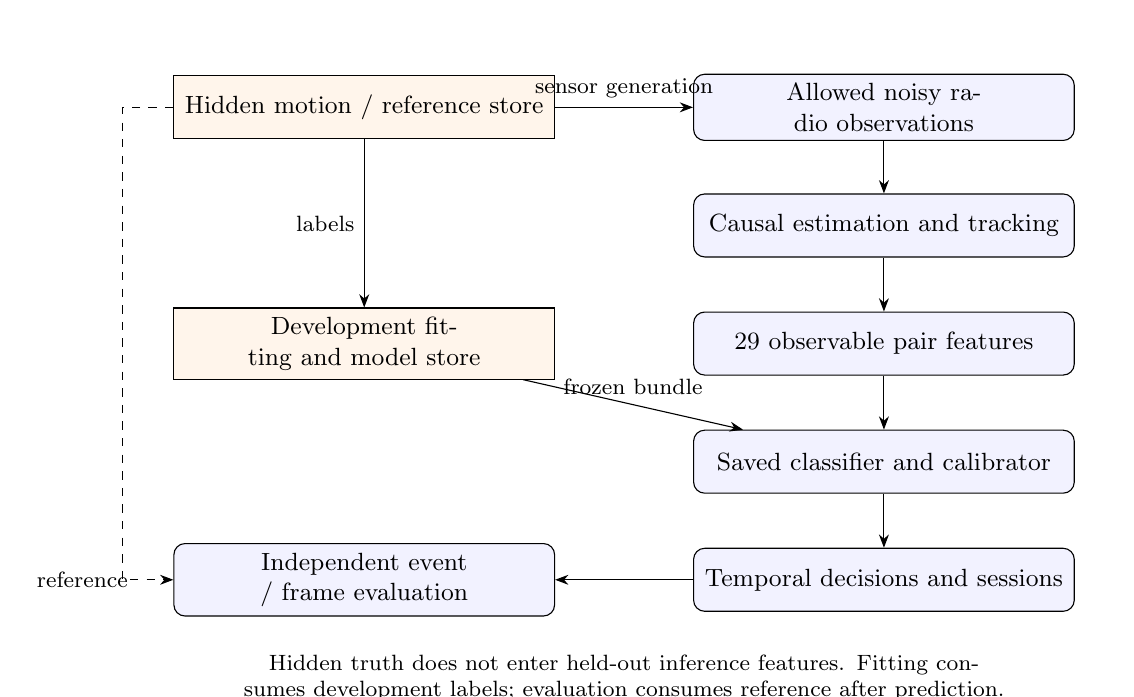
\begin{tikzpicture}[font=\small,>=Stealth,
box/.style={draw,rounded corners,fill=blue!5,align=center,text width=4.6cm,minimum height=.8cm},
store/.style={draw,fill=orange!8,align=center,text width=4.6cm,minimum height=.8cm}]
\node[store] (truth) at (0,0){Hidden motion / reference store};
\node[box] (obs) at (6.6,0){Allowed noisy radio observations};
\node[box] (estimate) at (6.6,-1.5){Causal estimation and tracking};
\node[box] (features) at (6.6,-3){29 observable pair features};
\node[box] (predict) at (6.6,-4.5){Saved classifier and calibrator};
\node[box] (sessions) at (6.6,-6){Temporal decisions and sessions};
\node[box] (evaluate) at (0,-6){Independent event / frame evaluation};
\node[store] (models) at (0,-3){Development fitting and model store};
\draw[->] (truth)--node[above,font=\footnotesize]{sensor generation}(obs);
\draw[->] (obs)--(estimate);\draw[->] (estimate)--(features);
\draw[->] (features)--(predict);\draw[->] (predict)--(sessions);
\draw[->] (sessions)--(evaluate);
\draw[->] (truth)--node[left,font=\footnotesize]{labels}(models);
\draw[->] (models)--node[above,font=\footnotesize]{frozen bundle}(predict);
\draw[->,dashed] (truth.west) -- ++(-.65,0) |- node[pos=.65,left,font=\footnotesize]{reference}(evaluate.west);
\node[align=center,text width=12cm,font=\footnotesize] at (3.3,-7.25){Hidden truth does not enter held-out inference features. Fitting consumes development labels; evaluation consumes reference after prediction.};
\end{tikzpicture}
\caption{Research architecture and hidden/observable information separation}\label{fig:architecture}
\end{figure}


\subsection{System Components}
The main components are the movement generator, independent label constructor, observation generator, modality interface, causal measurement history, robust localizer, tracker, pair-feature builder, classifier/calibrator, temporal decoder, event evaluator, and artifact store. Each has a defined information boundary.

Movement and reference construction know true positions. Observation generation also uses those positions to synthesize measurements. Downstream inference sees measurements, public anchor metadata, and the map. The classifier sees observable features. The evaluator compares predictions with separately retained labels and sessions after prediction.

The original identity registry and dashboard remain companion prototype modules. They are not hidden sources of true room or person status for the main learned detector. A future combined deployment must define how authorized identity continuity is maintained across rotating broadcasts.

\subsection{Working of the Proposed System}
For each partition seed, the movement generator creates a continuous sampled trajectory and derives physical pair labels. The observation generator applies the ideal or wall-error setting, including noise and reception loss. Each modality then receives only its permitted evidence.

At each time sample, trailing histories filter measurements, localization estimates tag coordinates, and tracking combines current estimates with movement predictions. The feature builder describes each pair using estimated geometry, telemetry, agreement, diagnostics, and past histories. It also records whether the pair is currently eligible.

A fitted classifier produces a raw positive score, a separately fitted map calibrates that score, and the frozen threshold/decoder creates a binary temporal sequence. Consecutive positive runs spanning at least 30 seconds become predicted sessions. The independent evaluator matches them to reference sessions, calculates errors, and aggregates supported conditions within each seed before averaging seeds.

The report is generated from retained evidence. It does not create final values by editing dashboard displays or by replacing unfavorable test selections with later winners.

\section{High-Level Design}
The high-level design assigns sensing, estimation, learning, and evaluation distinct responsibilities. The separation is particularly important for a simulator: code that knows the hidden answer must not be reused as an inference shortcut. Figure references and module names below describe the implementation or explicitly marked companion architecture, not unbuilt hardware.


\begin{figure}[htbp]
\centering
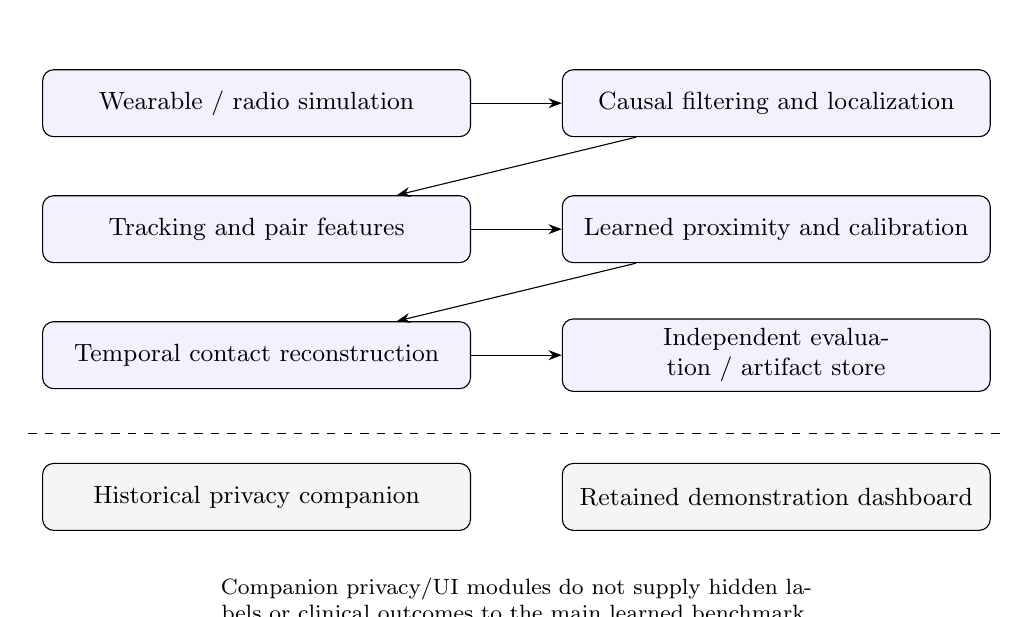
\begin{tikzpicture}[font=\small,>=Stealth,
box/.style={draw,rounded corners,fill=blue!5,align=center,text width=5.2cm,minimum height=.85cm}]
\node[box] (obs) at (0,0){Wearable / radio simulation};
\node[box] (infer) at (6.6,0){Causal filtering and localization};
\node[box] (feat) at (0,-1.6){Tracking and pair features};
\node[box] (ml) at (6.6,-1.6){Learned proximity and calibration};
\node[box] (session) at (0,-3.2){Temporal contact reconstruction};
\node[box] (eval) at (6.6,-3.2){Independent evaluation / artifact store};
\node[box,fill=gray!8] (privacy) at (0,-5){Historical privacy companion};
\node[box,fill=gray!8] (ui) at (6.6,-5){Retained demonstration dashboard};
\draw[->] (obs)--(infer);\draw[->] (infer)--(feat);\draw[->] (feat)--(ml);
\draw[->] (ml)--(session);\draw[->] (session)--(eval);
\draw[dashed] (-2.9,-4.2)--(9.5,-4.2);
\node[font=\footnotesize,align=center,text width=12cm] at (3.3,-6.3){Companion privacy/UI modules do not supply hidden labels or clinical outcomes to the main learned benchmark.};
\end{tikzpicture}
\caption{High-level component design; the demonstration and privacy companion are separate}\label{fig:highlevel}
\end{figure}


\subsection{Wearable Module}
The main experiment represents eight moving tags with synthetic identifiers. Tags supply the observation generator with positions internally, while the inference layer receives only generated radio measurements. Pair roles are shuffled so an identifier does not consistently encode a contact role.

The original prototype additionally models rotating pseudonyms. The v7 experiment does not implement a physical wristband, battery circuit, enclosure, secure provisioning service, or real antenna system. Such items are requirements of a future deployment rather than completed components of the simulation.

\subsection{BLE/RF Observation Module}
For tag i and gateway g, define dig(t) as their hidden separation and Wig(t) as an indicator that their connecting segment intersects the wall outside the doorway. RSSI is generated using

\begin{equation}
R_{ig}(t)=-50-25\log_{10}(\max\{0.1,d_{ig}(t)\})+6u_{ig}(t)+\beta_i-LW_{ig}(t)
\label{eq:source2}
\end{equation}

Distances are in metres and RSSI is in dBm. The reference value is -50 dBm and path-loss exponent is 2.5. The unit-variance state follows u(t) = rhou(t-1) + sqrt(1-rho squared)epsilon(t), with independent standard-normal innovations. A separate state generates angular error. In the wall condition, device bias betai is drawn once per recording from a zero-mean Gaussian with 2 dB standard deviation; wall attenuation is 6 dB and rho = 0.8. The ideal condition sets these biases and correlation to zero.

The bearing is the true gateway-to-tag angle relative to gateway orientation plus a 5 degrees stochastic error, a persistent gateway orientation bias, and a wall angular bias, wrapped into the circular interval. Orientation-bias standard deviation is 2 degrees and wall bias is 8 degrees in the wall condition, and both are zero in the ideal condition. Independent packet loss is 10\%; observations below -95 dBm are dropped. The wall condition also draws burst starts with probability 0.008 per link per second and suppresses that link for three seconds. This is an abstract reception process without RF interference or a BLE packet scheduler.

The label LOS denotes the ideal sensor-error setting without modeled wall penalties; it does not assert that every link has physical line of sight in the two-room geometry. The second setting is named wall multipath and introduces correlated errors and biases. These distributions are engineering assumptions chosen for controlled contrasts, not measurements fitted from hospital radios. Table~\ref{tab:channel} lists the channel parameters so that conclusions can be interpreted conditionally.

\begingroup
\small\setstretch{1.05}\setlength{\tabcolsep}{3pt}
\begin{longtable}{>{\raggedright\arraybackslash}p{0.430\linewidth}>{\raggedright\arraybackslash}p{0.250\linewidth}>{\raggedright\arraybackslash}p{0.260\linewidth}}
\caption{Assumed sensor and reception parameters}\label{tab:channel}\\
\toprule
\textbf{Parameter} & \textbf{Ideal setting} & \textbf{Wall setting}\\
\midrule
\endfirsthead
\toprule
\textbf{Parameter} & \textbf{Ideal setting} & \textbf{Wall setting}\\
\midrule
\endhead
\bottomrule
\endfoot
RSSI noise SD (d\allowbreak{}B) & 6 & 6\\
RSSI and angular AR correlation & 0 & 0.8\\
Persistent device RSSI bias SD (d\allowbreak{}B) & 0 & 2\\
Wall attenuation (d\allowbreak{}B) & 0 & 6\\
Bearing noise SD (degrees) & 5 & 5\\
Gateway orientation bias SD (degrees) & 0 & 2\\
Wall bearing bias (degrees) & 0 & 8\\
Independent packet loss & 0.10 & 0.10\\
Sensitivity floor (d\allowbreak{}Bm) & -95 & -95\\
Burst-start probability per link per second & 0 & 0.008\\
Burst length (s) & 0 & 3\\
PBR phase noise SD (rad) & 0.25 & 0.50\\
Blocked-link reflected amplitude /\allowbreak{} excess path & 0 /\allowbreak{} 0 & 1.4 /\allowbreak{} 2 m\\
RTT elapsed-time noise SD (ns) & 10 & 10\\
UWB interval noise SD (ns) & 0.4 & 0.4\\
RTT blocked-link bias (m) & 0 & 1.5\\
UWB blocked-link bias (m) & 0 & 0.8\\
Persistent PBR /\allowbreak{} RTT /\allowbreak{} UWB range-bias SD (m) & 0.15 /\allowbreak{} 0.30 /\allowbreak{} 0.10 & 0.15 /\allowbreak{} 0.30 /\allowbreak{} 0.10\\
\end{longtable}
\endgroup


The PBR simulator generates 72 synthetic tones fk = 2402 MHz + k MHz for k = 0,...,71. This uniform tone sequence is not the exact Bluetooth channel map. A reciprocal two-path channel has a direct component and, on blocked links, a reflected component with excess path length 2 m and relative amplitude 1.4. The reflected component has an additional fixed 0.7 radian phase. The combined round-trip phase is twice the channel phase, plus a link-specific nuisance offset and independent phase noise:

\begin{equation}
\begin{aligned}\phi_k=\operatorname{wrap}\bigl[2\arg\{&\exp(j2\pi f_kd/c)\\&+\alpha\exp(j[2\pi f_k(d+\ell)/c+0.7])\}+\phi_0+\eta_k\bigr]\end{aligned}
\label{eq:source3}
\end{equation}

The amplitude alpha is zero on unblocked links and in the ideal condition. Phase-noise standard deviation is 0.25 radian in the ideal condition and 0.5 radian in the wall condition. A link-specific distance-calibration bias has standard deviation 0.15 m. Under the simulator's positive-phase convention, the estimator unwraps neighboring phases, fits a least-squares slope sphi against frequency in hertz, and converts that slope to distance:

\begin{equation}
\widehat d_{\mathrm{PBR}}=\frac{c s_\phi}{4\pi},\qquad c=299\,792\,458\ \mathrm{m/s}
\label{eq:source4}
\end{equation}

The phase-fit residual is observable but is not a truth-based multipath label. Negative or nonfinite estimates are unavailable. Ideal reciprocity and a constant offset across tones simplify oscillator behavior; the simulation does not model real controller measurements or standards compliance.

Corrected RTT uses an elapsed time and a reported turnaround of \(10^6\) ns. Elapsed-time noise has standard deviation 10 ns; link calibration bias has standard deviation 0.3 m; blocked links receive a further assumed 1.5 m bias in the wall condition. With intervals expressed in seconds, the estimator is

\begin{equation}
\widehat d_{\mathrm{RTT}}=\frac{c}{2}(T_{\mathrm{elapsed}}-T_{\mathrm{turnaround}})
\label{eq:source5}
\end{equation}

UWB uses ideal double-sided two-way timing with clock skews of +20 ppm and -15 ppm, turnaround intervals of \(5\times10^5\) and \(7\times10^5\) ns, independent interval noise of 0.4 ns standard deviation, and a link calibration bias of 0.1 m standard deviation. The assumed blocked-link bias is 0.8 m in the wall condition. For round intervals R\_A,R\_B and reply intervals D\_A,D\_B in seconds,

\begin{equation}
\widehat T_{\mathrm{ToF}}=\frac{R_AR_B-D_AD_B}{R_A+R_B+D_A+D_B},\qquad \widehat d_{\mathrm{UWB}}=c\widehat T_{\mathrm{ToF}}
\label{eq:source6}
\end{equation}

The PBR\_RTT branch returns the PBR distance only when RTT is valid and the disagreement is at most three times sqrt(0.2 squared + 1.5 squared) m. Otherwise, it abstains. This is a coarse consistency gate. It neither combines estimates into a new distance estimator nor establishes resistance to adversarial ranging; a shared bias can pass the gate.

Active ranging follows round-robin service with four client slots per gateway per second. The same selected tag batch is used across gateways and ranging methods. With eight clients, a tag is scheduled every two seconds before reception loss. All radio branches share the received BLE-link mask to control observation availability. Consequently, UWB coverage and Bluetooth Channel Sounding procedure airtime are not independently characterized.

Equalizing slots removes one experimental confound but imposes an application-level service assumption rather than a measured technology capacity. Conditional comparisons must therefore separate distance-error assumptions from update availability. A prior, separately versioned scheduling campaign supplies supporting load observations in the supporting-results section; its additional clients consume slots but have no extra physical trajectories.

\subsection{Edge Processing Module}
RSSI uses a causal five-second median history, and bearings use a causal circular mean over the same period. RSSI/angular localization minimizes a Huber loss \cite{ref13} on standardized log-distance and circular-bearing residuals. The Huber cutoff is 1.5. The solver uses multiple public-anchor-derived initial positions, at most 30 Gauss--Newton iterations, regularized normal equations, and backtracking. At least three RSSI observations or two angular observations are required. No true room or hidden bounding position constrains this optimization.

Ranging branches use valid current ranging links whose values are median-filtered using their preceding five-second histories. At least three links are needed for robust range localization. The assumed residual scales are 0.2 m for PBR, PBR\_RTT and UWB and 1.5 m for RTT; these are estimator parameters, not measured accuracy. The numerical optimizer otherwise uses the same Huber cutoff and multistart principle.

Each coordinate is then tracked with a constant-velocity Kalman filter \cite{ref14}. Acceleration variance is 0.08. Position-measurement variance is 4 for RSSI and RTT, 0.64 for RSSI/angular fusion, and 0.16 for the other ranging configurations, in squared metre units. Initial velocity is zero with variance 1. Predictions expire when more than three seconds have elapsed since a usable localization measurement. These covariance choices are fixed engineering assumptions, not covariances estimated from held-out truth.

The earlier edge pipeline also includes packet validation, normalization, deduplication, temporal pair evidence, and sessionization. Those functions provide a modular acquisition-processing design. The main trained campaign reuses causal estimation mechanisms from the separately versioned angular/contact/ranging modules and performs offline generation and fitting.

Median filtering suppresses some isolated outliers, while a circular mean respects angular wrapping. Huber loss limits the influence of very large standardized residuals. Kalman tracking maintains a movement estimate between updates, but expires it when it becomes stale. Each is a useful mechanism whose fixed parameters remain part of the experiment's assumptions.

\subsection{Contact Reconstruction Module}
The 29-dimensional pair feature vector describes estimated separation/room, position availability, telemetry age, common receivers, RSSI agreement and counts, angular agreement, range-profile differences, fit diagnostics, and past 10/30-second contact histories. Features are symmetric under exchanging the pair's members. Estimated distance is capped at 30 m. Numeric features are rounded to three decimal places and stored as little-endian float32. The feature-schema table defines every column and its units.

Availability requires tracked positions for both tags and recent BLE telemetry for each, no older than three seconds. Unavailable pair-distance and room fields are zero with an explicit availability flag, and inference output is forced nonpositive. Missing modality-specific diagnostics also use zero; their interpretation must be considered with the observation budget and availability. The gate prevents a model from declaring contacts when its required geometry is unavailable, but necessarily sacrifices possible recall. It is not evidence that a missing observation means physical separation.

The feature histories include the current sample and never inspect future frames. Ten- and thirty-second positive fractions refer to a fixed estimated 2 m same-room rule, not true labels. The room ablation removes only the estimatedSameRoom column; remaining positions and signal profiles can still encode room-related information. It is therefore not a comprehensive map-free ablation.

\begingroup
\small\setstretch{1.05}\setlength{\tabcolsep}{3pt}
\begin{longtable}{>{\raggedright\arraybackslash}p{0.045\linewidth}>{\raggedright\arraybackslash}p{0.280\linewidth}>{\raggedright\arraybackslash}p{0.520\linewidth}>{\raggedright\arraybackslash}p{0.095\linewidth}}
\caption{Table A1 Observable feature schema}\label{tab:features}\\
\toprule
\textbf{No} & \textbf{Column name} & \textbf{Definition} & \textbf{Unit}\\
\midrule
\endfirsthead
\toprule
\textbf{No} & \textbf{Column name} & \textbf{Definition} & \textbf{Unit}\\
\midrule
\endhead
\bottomrule
\endfoot
1 & estimated\allowbreak{}Distance & Estimated separation capped at 30; zero if unavailable & m\\
2 & estimated\allowbreak{}Same\allowbreak{}Room & Same side of public wall from estimated positions & binary\\
3 & pair\allowbreak{}Position\allowbreak{}Available & Tracked pair positions and BLE ages at most 3 s & binary\\
4 & min\allowbreak{}Telemetry\allowbreak{}Age & Smaller latest-telemetry age; 30 if none & s\\
5 & max\allowbreak{}Telemetry\allowbreak{}Age & Larger latest-telemetry age; 30 if none & s\\
6 & common\allowbreak{}Receivers & Common receivers in five-second telemetry histories & count\\
7 & min\allowbreak{}Mean\allowbreak{}Rssi & Smaller device mean of receiver-median RSSI & d\allowbreak{}Bm\\
8 & max\allowbreak{}Mean\allowbreak{}Rssi & Larger device mean of receiver-median RSSI & d\allowbreak{}Bm\\
9 & rssi\allowbreak{}Mean\allowbreak{}Difference & Absolute mean signed RSSI difference on common receivers & d\allowbreak{}B\\
10 & centered\allowbreak{}Rssi\allowbreak{}Profile\allowbreak{}Difference & Mean absolute common-receiver RSSI differences after offset removal & d\allowbreak{}B\\
11 & rssi\allowbreak{}Profile\allowbreak{}Max\allowbreak{}Difference & Maximum offset-removed RSSI profile difference & d\allowbreak{}B\\
12 & min\allowbreak{}Packet\allowbreak{}Count & Smaller received-observation count over five-second histories & count\\
13 & max\allowbreak{}Packet\allowbreak{}Count & Larger received-observation count over five-second histories & count\\
14 & mean\allowbreak{}Angular\allowbreak{}Difference & Mean circular angular difference on common enabled receivers & rad\\
15 & max\allowbreak{}Angular\allowbreak{}Difference & Maximum circular angular difference & rad\\
16 & mean\allowbreak{}Range\allowbreak{}Profile\allowbreak{}Difference & Mean absolute common-anchor range difference & m\\
17 & max\allowbreak{}Range\allowbreak{}Profile\allowbreak{}Difference & Maximum absolute common-anchor range difference & m\\
18 & mean\allowbreak{}Range\allowbreak{}Fit\allowbreak{}Residual & Mean absolute observed-versus-estimated range residual & m\\
19 & mean\allowbreak{}Phase\allowbreak{}Fit\allowbreak{}Residual & Mean unwrapped phase-slope residual on current PBR links & rad\\
20 & mean\allowbreak{}Pbr\allowbreak{}Rtt\allowbreak{}Disagreement & Mean PBR/\allowbreak{}RTT disagreement on accepted combined links & m\\
21 & distance\allowbreak{}Mean10 & Mean available separation in preceding ten seconds & m\\
22 & distance\allowbreak{}Std10 & SD of available separation in preceding ten seconds & m\\
23 & distance\allowbreak{}Mean30 & Mean available separation in preceding thirty seconds & m\\
24 & positive\allowbreak{}Fraction10 & Fixed estimated 2 m same-room positives /\allowbreak{} history samples over 10 s & 0--1\\
25 & positive\allowbreak{}Fraction30 & Same fraction over 30 s & 0--1\\
26 & available\allowbreak{}Fraction10 & Available samples /\allowbreak{} history samples over 10 s & 0--1\\
27 & available\allowbreak{}Fraction30 & Same fraction over 30 s & 0--1\\
28 & distance\allowbreak{}Change10 & Last minus first available distance in ten-second history & m\\
29 & rssi\allowbreak{}Profile\allowbreak{}Difference\allowbreak{}Mean10 & Mean offset-removed RSSI profile difference in ten-second history & d\allowbreak{}B\\
\end{longtable}
\endgroup


Strict decoding declares a positive frame when p(t) >= tau and the pair is eligible. Occupancy decoding requires at least seven eligible threshold-positive samples in the full ten-frame causal window, with eligibility at the current frame. The first nine frames are nonpositive because their windows are incomplete:

\begin{equation}
b(t)=e(t)\,\mathbf{1}\!\left\{\sum_{u=t-9}^{t}e(u)\mathbf{1}[p(u)\geq\tau]\geq7\right\},\quad t\geq9
\label{eq:source8}
\end{equation}

The current sample need not itself exceed the probability threshold if the occupancy requirement is met. Predicted contacts are maximal consecutive positive decoded runs spanning at least 30 s. An unavailable current estimate breaks a run. The earliest confirmation time assigned to a qualified run is its start plus 30 s. Session boundaries are reconstructed retrospectively from causal decisions; they are not available in full at initial confirmation.

Validation searches probability thresholds \{0.2,0.35,0.5,0.65,0.8\} and both decoders, optimizing reconstructed-contact F1 rather than frame accuracy. Within policy search, ties favor fewer false positives, more matches, a higher threshold, and strict decoding. Candidate hyperparameters and the primary full family are compared using validation F1, then fewer false positives and more matches; a residual exact tie retains earlier enumeration order. The model chosen on validation remains primary even if another family scores higher on the final test.

\subsection{Learned Contact Classification and Probability Calibration}
The module produces calibrated probabilities of instantaneous synthetic same-room proximity; it is not a clinical exposure or infection-risk model.

We fit logistic regression, random forest \cite{ref15}, histogram gradient boosting [11,16], and Gaussian naive Bayes separately for each observation configuration. Table~\ref{tab:models} gives the complete search grids. Standardization is fitted on training data for logistic regression and Gaussian Bayes. Balanced class weights are used for logistic regression, random forest, and boosted trees. The Gaussian model learns empirical class priors, conditional means and variances. No synthetic positive oversampling is applied.

\begingroup
\small\setstretch{1.05}\setlength{\tabcolsep}{3pt}
\begin{longtable}{>{\raggedright\arraybackslash}p{0.180\linewidth}>{\raggedright\arraybackslash}p{0.300\linewidth}>{\raggedright\arraybackslash}p{0.460\linewidth}}
\caption{Declared classifier search grids}\label{tab:models}\\
\toprule
\textbf{Family} & \textbf{Candidate settings} & \textbf{Fixed fitting settings}\\
\midrule
\endfirsthead
\toprule
\textbf{Family} & \textbf{Candidate settings} & \textbf{Fixed fitting settings}\\
\midrule
\endhead
\bottomrule
\endfoot
Logistic & C  in  \{0.1, 1\} & Standardized; balanced weights; max 2,000 iterations\\
Random forest & Depth  in  \{8, 12\} & 64 trees; leaf minimum 25; balanced weights\\
Histogram boosting & Leaves  in  \{15, 31\} & 80 iterations; leaf minimum 50; L2 = 0.1; balanced weights; no early stopping\\
Gaussian Bayes & Variance smoothing  in  \(\{10^{-6},10^{-3}\}\) & Standardized; empirical class priors\\
\end{longtable}
\endgroup


Every candidate's raw positive probability q is clipped to \([10^{-6},1-10^{-6}]\), transformed to log odds, and passed through a separately fitted sigmoid map. The calibration recordings are disjoint from training and validation. An unweighted logistic map with C = 100 and at most 2,000 iterations preserves their natural class prevalence:

\begin{equation}
p(t)=\sigma\!\left(a\log\frac{q(t)}{1-q(t)}+b\right),\qquad \sigma(v)=\frac{1}{1+\exp(-v)}
\label{eq:source7}
\end{equation}

Calibration is fitted using eligible pair-frames. Candidate classifiers themselves are fitted to all sampled training pair-frames, including those with unavailable estimates; the explicit gate still forces unavailable prediction probabilities to zero. Calibration here concerns instantaneous synthetic proximity, not qualified-session validity. Its performance is measured on full held-out recordings, including gated frames.

A two-state Markov extension estimates transition probabilities from consecutive full training labels, with add-one smoothing. Both matched channel-condition copies of the training labels contribute to these counts. The initial state probability is the training-frame positive prevalence. Let s(t-1) be the previous filtered probability and a01,a11 the learned transition probabilities. The predicted state probability is s-(t) = [1-s(t-1)]a01 + s(t-1)a11. We approximate emission log-likelihood evidence by subtracting the eligible calibration prevalence pi\_cal from the calibrated classifier log odds:

\begin{equation}
s(t)=\sigma\!\left(\operatorname{logit}[s^-(t)]+\operatorname{logit}[p(t)]-\operatorname{logit}[\pi_{\mathrm{cal}}]\right)
\label{eq:source9}
\end{equation}

For unavailable frames, the emission increment is zero and the output is gated to zero, although the internal state propagates. Threshold and decoder are selected on validation. Overlapping feature histories violate the ideal independent-emission assumption, so this extension is evaluated as an approximation and its outputs are not assumed calibrated.

Two ablations refit the validation-selected full family's hyperparameter configuration after removing the nine contact-history columns or the estimated-room column. They receive their own calibration and threshold/decoder selection. Seven detector bundles per observation budget are retained: four full families, the Markov extension, and two ablations. Thus 49 saved bundles include shared base classifiers in the Markov variants; they are not 49 independent datasets.

\subsection{Privacy Module}
The companion privacy design separates broadcast pseudonyms from a protected identity mapping. Authorized processing can resolve identifiers to maintain records, while public observations do not need direct personal identities. Rotation experiments consider collision, linkability, and the effect of identifier changes on contact continuity.

The existing authorization context is an application interface; it must not be described as a fully audited authentication service. Deterministic simulation pseudonyms provide reproducibility rather than secrecy. Keyed HMAC generation is implemented, but full key lifecycle, endpoint security, transport security, and institutional governance are not evaluated by the main trained study.

Stable identity association is necessary to build causal histories. The final contact evaluation does not quantify the additional error introduced when that association must be recovered across real rotating identifiers. That remains a separate integration experiment.

\subsection{Dashboard Module}
The React demonstration presents simulated movement and project modules through a graphical interface. Its purpose is to help users inspect the intended workflow and understand reconstructed contact records. Historical risk terminology and live heuristics must not be substituted for the main v7 result tables.

A research-facing output view should identify the run version, modality, selected family, threshold, decoder, and contact interval, and should distinguish probability from infection risk. It should display missing evidence and uncertainty rather than silently treating absent observations as physical separation.

The report contains vector views of the frozen research evidence and actual captured screens of the retained demonstration. The two forms of output are explicitly distinguished. The screenshots illustrate the interface, not validated hospital or infection outcomes.

\section{Use-Case Diagram}
The use-case view distinguishes the implemented research workflow from an eventual hospital workflow. Researchers generate and verify experiments; developers test code boundaries; students inspect the demonstration. A future authorized investigator would review contacts after a separately validated operational deployment.


\begin{figure}[htbp]
\centering
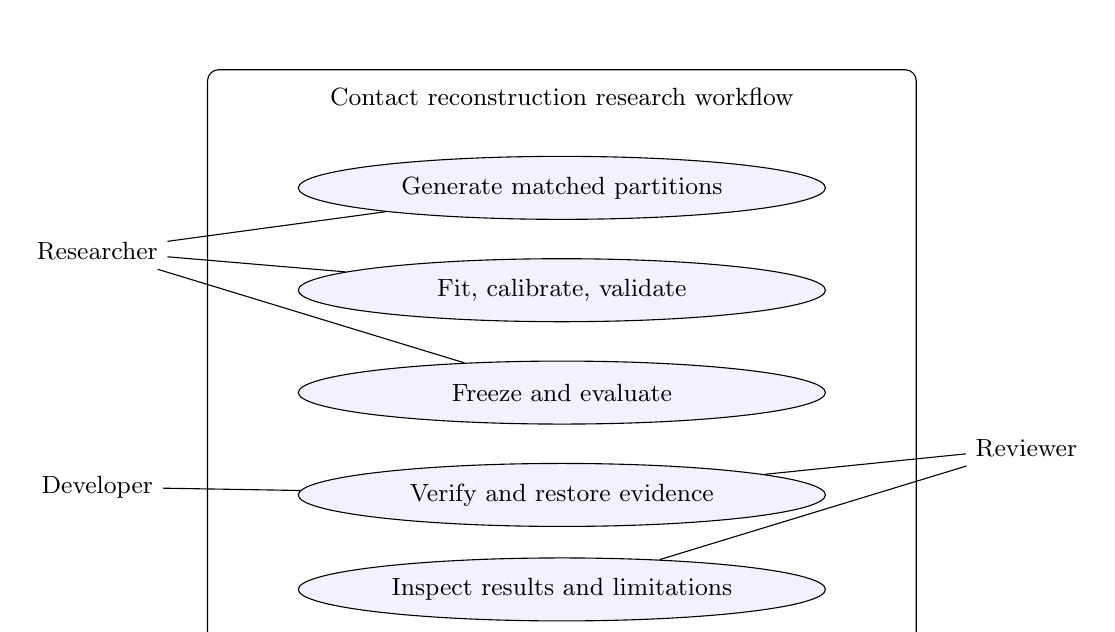
\begin{tikzpicture}[font=\small,>=Stealth,
uc/.style={ellipse,draw,fill=blue!5,align=center,text width=4.5cm,minimum height=.8cm}]
\draw[rounded corners] (0,.8) rectangle (9,-6.5);
\node at (4.5,.45){Contact reconstruction research workflow};
\node[uc] (gen) at (4.5,-.7){Generate matched partitions};
\node[uc] (fit) at (4.5,-2){Fit, calibrate, validate};
\node[uc] (test) at (4.5,-3.3){Freeze and evaluate};
\node[uc] (check) at (4.5,-4.6){Verify and restore evidence};
\node[uc] (report) at (4.5,-5.8){Inspect results and limitations};
\node[align=center] (researcher) at (-1.4,-1.5){Researcher};
\node[align=center] (developer) at (-1.4,-4.5){Developer};
\node[align=center] (reviewer) at (10.4,-4){Reviewer};
\draw (researcher)--(gen);\draw (researcher)--(fit);\draw (researcher)--(test);
\draw (developer)--(check);\draw (reviewer)--(check);\draw (reviewer)--(report);
\end{tikzpicture}
\caption{Use-case view of implemented research activities}\label{fig:usecase}
\end{figure}


\subsection*{Actors and Their Responsibilities}
The researcher fixes a protocol, generates development data, fits models, freezes selections, evaluates held-out data, and interprets limitations. The developer maintains the information boundaries and runs regression checks. The reviewer checks provenance, numerical consistency, comparator fairness, and whether conclusions exceed the evidence.

The student or demonstration user can inspect project concepts without treating display values as clinical decisions. An authorized infection-control investigator is a proposed operational actor, not a participant in the completed synthetic study. No patient or hospital employee provided personal data for v7.

\subsection*{Major Use Cases}
Major implemented use cases are creating a fresh simulation partition, training/calibrating/selecting a model, running held-out evaluation, applying feature-only inference, independently verifying saved labels and metrics, restoring release evidence, and generating tables and figures.

Future operational use cases include assigning wearables, managing keys, authorizing identity resolution, reviewing contacts, and integrating with institutional records. These are separated from completed experimental functions to prevent a design diagram from being interpreted as deployment evidence.

\section{Data Flow Diagram}
The data-flow view makes hidden and observable stores explicit. The reference store feeds fitting labels and post-prediction evaluation; it does not feed inference features. The model store receives fitted development outputs and supplies held-out prediction. The result store preserves per-recording outputs and run metadata.

\subsection{DFD Level 0}
At the context level, protocol and synthetic observations enter the reconstruction system, and predicted sessions and evaluation artifacts leave it. Independent reference sessions enter only the evaluation path. A human researcher reviews the resulting evidence and its assumptions.


\begin{figure}[htbp]
\centering
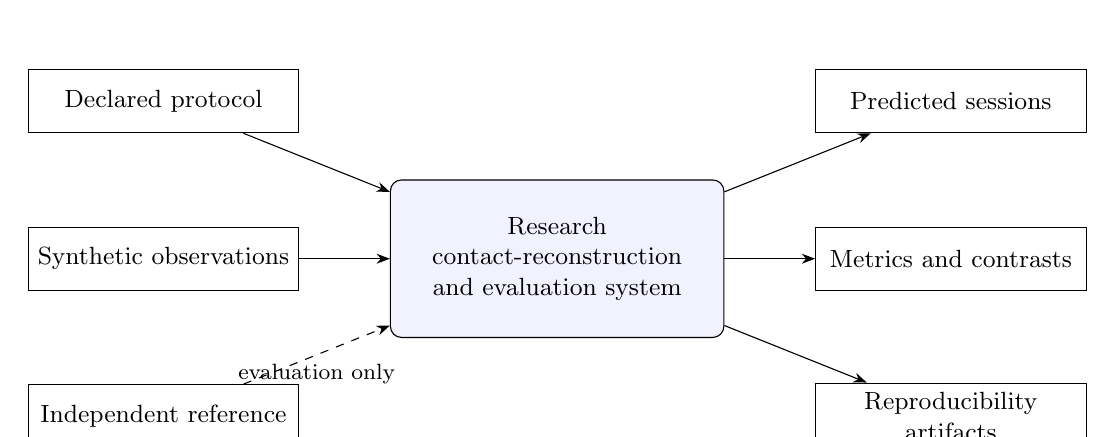
\begin{tikzpicture}[font=\small,>=Stealth,
box/.style={draw,align=center,text width=3.2cm,minimum height=.8cm},
process/.style={draw,rounded corners,fill=blue!5,align=center,text width=4cm,minimum height=2cm}]
\node[box] (protocol) at (0,0){Declared protocol};
\node[box] (obs) at (0,-2){Synthetic observations};
\node[box] (reference) at (0,-4){Independent reference};
\node[process] (system) at (5,-2){Research\\contact-reconstruction\\and evaluation system};
\node[box] (contacts) at (10,0){Predicted sessions};
\node[box] (metrics) at (10,-2){Metrics and contrasts};
\node[box] (evidence) at (10,-4){Reproducibility artifacts};
\draw[->] (protocol)--(system);\draw[->] (obs)--(system);
\draw[->,dashed] (reference)--node[below,font=\footnotesize]{evaluation only}(system);
\draw[->] (system)--(contacts);\draw[->] (system)--(metrics);\draw[->] (system)--(evidence);
\end{tikzpicture}
\caption{Data-flow context diagram}\label{fig:dfd0}
\end{figure}


\subsection{DFD Level 1}
The expanded data flow begins with protocol-controlled motion and sensor generation. Causal estimation produces positions and diagnostics; the feature builder produces fixed-order arrays; development fitting writes model bundles; held-out inference writes probabilities and sessions; independent evaluation writes metrics and grouped contrasts.

Labels are stored separately from features, even though both originate from one simulated world. The public map and anchor locations are allowed metadata. True rooms, positions, pair distances, contact-role identities, and future status are prohibited predictor inputs.


\begin{figure}[htbp]
\centering
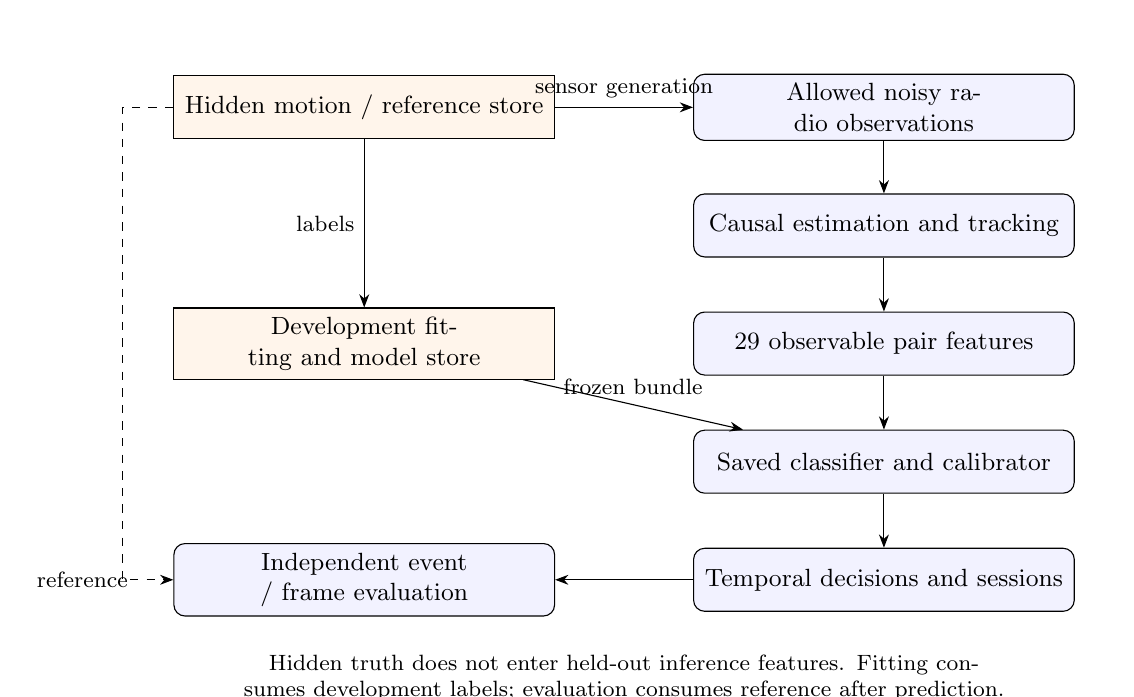
\begin{tikzpicture}[font=\small,>=Stealth,
box/.style={draw,rounded corners,fill=blue!5,align=center,text width=4.6cm,minimum height=.8cm},
store/.style={draw,fill=orange!8,align=center,text width=4.6cm,minimum height=.8cm}]
\node[store] (truth) at (0,0){Hidden motion / reference store};
\node[box] (obs) at (6.6,0){Allowed noisy radio observations};
\node[box] (estimate) at (6.6,-1.5){Causal estimation and tracking};
\node[box] (features) at (6.6,-3){29 observable pair features};
\node[box] (predict) at (6.6,-4.5){Saved classifier and calibrator};
\node[box] (sessions) at (6.6,-6){Temporal decisions and sessions};
\node[box] (evaluate) at (0,-6){Independent event / frame evaluation};
\node[store] (models) at (0,-3){Development fitting and model store};
\draw[->] (truth)--node[above,font=\footnotesize]{sensor generation}(obs);
\draw[->] (obs)--(estimate);\draw[->] (estimate)--(features);
\draw[->] (features)--(predict);\draw[->] (predict)--(sessions);
\draw[->] (sessions)--(evaluate);
\draw[->] (truth)--node[left,font=\footnotesize]{labels}(models);
\draw[->] (models)--node[above,font=\footnotesize]{frozen bundle}(predict);
\draw[->,dashed] (truth.west) -- ++(-.65,0) |- node[pos=.65,left,font=\footnotesize]{reference}(evaluate.west);
\node[align=center,text width=12cm,font=\footnotesize] at (3.3,-7.25){Hidden truth does not enter held-out inference features. Fitting consumes development labels; evaluation consumes reference after prediction.};
\end{tikzpicture}
\caption{Expanded observable research data flow}\label{fig:dfd1}
\end{figure}


\section{Class Diagram}
The implementation mixes object-oriented and functional components. The class view therefore includes actual classes alongside explicitly labeled functional modules, rather than inventing a hierarchy of unimplemented services. FeatureBuilder owns telemetry and pair histories; CausalMeasurements owns filtered measurement histories; CausalTracker maintains motion state. Python fitting and metrics are principally module-level functions.


\begin{figure}[htbp]
\centering
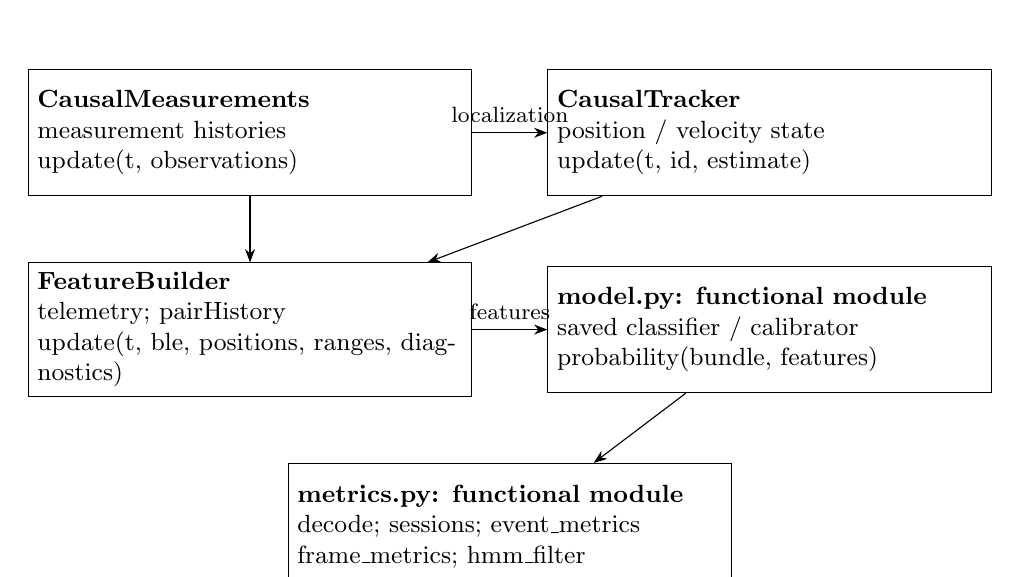
\begin{tikzpicture}[font=\small,>=Stealth,
box/.style={draw,rectangle,align=left,text width=5.4cm,minimum height=1.6cm}]
\node[box] (filter) at (0,0){\textbf{CausalMeasurements}\\measurement histories\\update(t, observations)};
\node[box] (tracker) at (6.6,0){\textbf{CausalTracker}\\position / velocity state\\update(t, id, estimate)};
\node[box] (features) at (0,-2.5){\textbf{FeatureBuilder}\\telemetry; pairHistory\\update(t, ble, positions, ranges, diagnostics)};
\node[box] (models) at (6.6,-2.5){\textbf{model.py: functional module}\\saved classifier / calibrator\\probability(bundle, features)};
\node[box] (metrics) at (3.3,-5){\textbf{metrics.py: functional module}\\decode; sessions; event\_metrics\\frame\_metrics; hmm\_filter};
\draw[->] (filter)--node[above,font=\footnotesize]{localization}(tracker);
\draw[->] (filter)--(features);\draw[->] (tracker)--(features);
\draw[->] (features)--node[above,font=\footnotesize]{features}(models);
\draw[->] (models)--(metrics);
\end{tikzpicture}
\caption{Actual classes and functional modules in the research pipeline}\label{fig:classes}
\end{figure}


\section{Sequence Diagram}
For one sampled instant, the generator supplies current allowed measurements to filtering and estimation. The tracker updates available positions, the feature builder emits pair inputs, and the saved bundle produces calibrated probability. The temporal decoder retains state over frames. Once a run qualifies, a session can be confirmed; complete boundaries are known after the run ends.

The evaluator compares stored predictions with independent reference sessions after inference. The sequence is causal at prediction time even though final interval summaries are assembled retrospectively.


\begin{figure}[htbp]
\centering
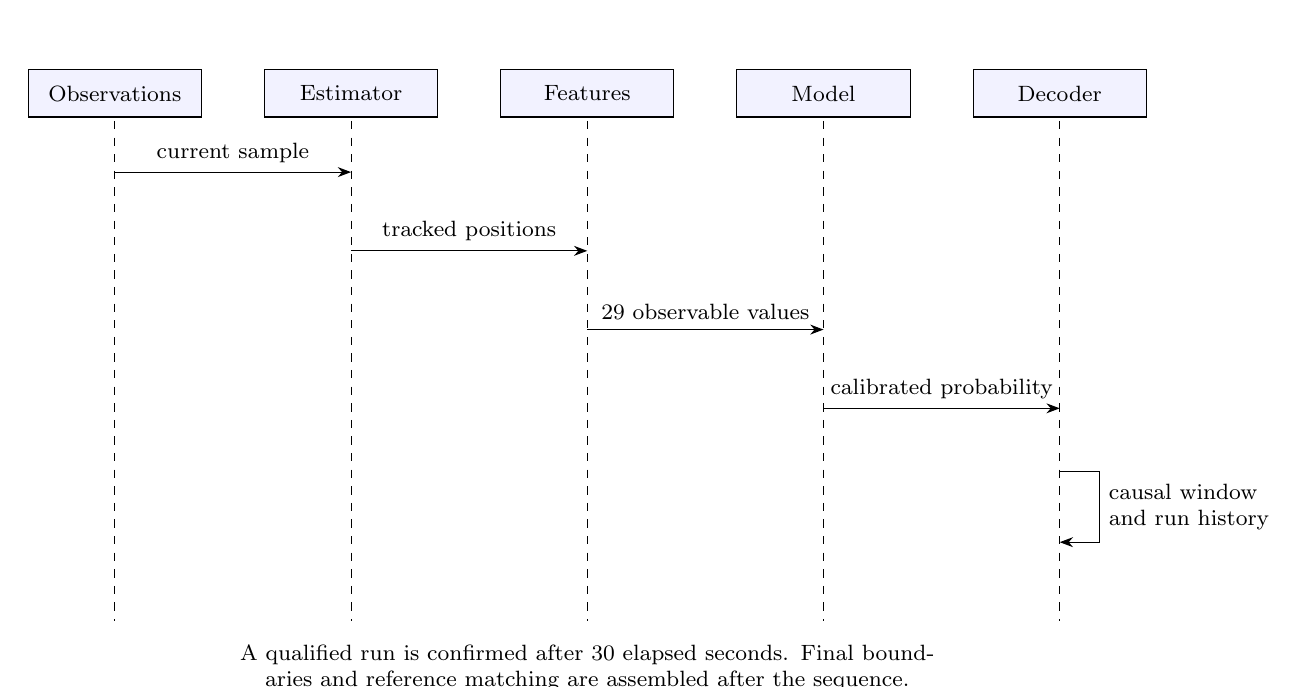
\begin{tikzpicture}[font=\footnotesize,>=Stealth]
\foreach \x/\name in {0/Observations,3/Estimator,6/Features,9/Model,12/Decoder}{
\node[draw,fill=blue!5,align=center,minimum width=2.2cm,minimum height=.6cm] at (\x,0){\name};
\draw[dashed] (\x,-.35)--(\x,-6.7);}
\draw[->] (0,-1)--node[above]{current sample}(3,-1);
\draw[->] (3,-2)--node[above]{tracked positions}(6,-2);
\draw[->] (6,-3)--node[above]{29 observable values}(9,-3);
\draw[->] (9,-4)--node[above]{calibrated probability}(12,-4);
\draw[->] (12,-4.8)--(12.5,-4.8)--node[right,align=left]{causal window\\and run history}(12.5,-5.7)--(12,-5.7);
\node[align=center,text width=12cm] at (6,-7.3){A qualified run is confirmed after 30 elapsed seconds. Final boundaries and reference matching are assembled after the sequence.};
\end{tikzpicture}
\caption{Causal observation-to-session sequence with post-prediction evaluation}\label{fig:sequence}
\end{figure}


\section{Implementation Details}
JavaScript modules generate the movement, observations, and features. Python with scikit-learn performs fitting, calibration, held-out evaluation, and numerical reporting. The original application uses TypeScript and React. The environments are intentionally separate so research dependencies and demonstration dependencies are identifiable.

\begingroup
\small\setstretch{1.05}\setlength{\tabcolsep}{3pt}
\begin{longtable}{>{\raggedright\arraybackslash}p{0.200\linewidth}>{\raggedright\arraybackslash}p{0.400\linewidth}>{\raggedright\arraybackslash}p{0.340\linewidth}}
\caption{Implementation modules and responsibilities}\label{tab:files}\\
\toprule
\textbf{Module} & \textbf{Location} & \textbf{Responsibility}\\
\midrule
\endfirsthead
\toprule
\textbf{Module} & \textbf{Location} & \textbf{Responsibility}\\
\midrule
\endhead
\bottomrule
\endfoot
Protocol and movement & research/\allowbreak{}ml-v7/\allowbreak{}protocol.mjs; scenarios.mjs & Partitions, assumptions, trajectories\\
Features & research/\allowbreak{}ml-v7/\allowbreak{}features.mjs & Symmetric observable input\\
Observation generation & research/\allowbreak{}contact-v5; research/\allowbreak{}ranging-v6 & RSSI, bearing, phase, and timing\\
Training & research/\allowbreak{}ml-v7/\allowbreak{}train.py & Fitting, calibration, selection\\
Decoding and metrics & research/\allowbreak{}ml-v7/\allowbreak{}metrics.py & Frames, sessions, matching, metrics\\
Verification & research/\allowbreak{}ml-v7/\allowbreak{}verify.py; final\_audit.py & Independent saved-artifact checks\\
Deployment demo & src/\allowbreak{}; public/\allowbreak{} & Retained React interface\\
Evidence recovery & scripts/\allowbreak{}restore\allowbreak{}Research\allowbreak{}Evidence.py & Verified archive restoration\\
\end{longtable}
\endgroup


\subsection{BLE Wearable Simulation}
The protocol fixes eight tags, 360 frames, the 2 m threshold, and the 30 s minimum span. The scenario module generates ward encounters, doorway rounds, and threshold encounters, while the held-out motion challenge uses independent waypoints. Each tag has a continuous sampled route, and role assignment is shuffled.

There are 28 unordered pairs per frame. The physical label array has shape 360 by 28. A feature array for one condition/modality has shape 360 by 28 by 29. Array order is timestamp-major then pair-major, with fixed predictor columns. Float32 features are rounded to three decimal places before storage; labels are unsigned 0/1 bytes.

\subsection{BLE/RF Simulation}
Radio generation is matched across observation budgets: one motion recording supplies the reference for both error conditions and every modality. The sensor modules inject assumed RSSI, bearing, phase, and timing errors and control packet availability. A branch cannot inspect hidden bearing fields unless its budget enables them, and PBR does not receive RTT diagnostics from the combined branch.

The phase sequence is abstract and uniformly spaced. Timing models use nanosecond intervals converted to seconds. UWB uses ideal DS-TWR rather than TDoA. All active branches share the imposed round-robin scheduling and BLE reception mask. These choices enable a controlled algorithm comparison but omit technology-specific RF capacities and real controller behavior.

Raw observations, true trajectories, labels, and feature arrays are retained separately. This permits later verification of the path from observations to results without retroactively relabeling old evidence.

\subsection{Edge Gateway Processing}
The processing stages are causal. RSSI and bearings use five-second histories; range filtering uses valid recent values when current links are available. Robust multistart localization estimates coordinates, and constant-velocity tracking bridges limited missing updates. Positions expire after more than three seconds without usable localization.

Features summarize pair geometry, receiver agreement, telemetry age, packet counts, fit residuals, and estimated contact histories. Missing geometry is explicitly gated. Distance zero is a sentinel when unavailable, not proof of zero separation. At least three RSSI/range links or two angular observations are needed by the corresponding localizer.

This implementation is evaluated offline. It does not supply a measured edge-device communication ratio, radio-to-server latency, or power budget in the final benchmark.

\subsection{Contact Session Reconstruction}
Training learns instantaneous same-room proximity, including brief encounters. Strict decoding uses current eligibility and the selected probability threshold. Occupancy decoding requires seven threshold-positive eligible samples in the full trailing ten-frame window and current eligibility. The current probability need not itself pass the threshold in occupancy mode.

Maximal consecutive decoded positive runs with end minus start at least 30 seconds become predictions. With one-second samples, 31 consecutive positive samples are the minimum. An unavailable current estimate breaks a run. Earliest confirmation is start plus 30 seconds, and the complete end boundary is later reconstructed from the sequence.

The same physical reference definition is used for all configurations. A tuned estimated-distance threshold of 2.5 or 3 m does not change the true 2 m label; it compensates for estimation error within a validation-selected rule.

\subsection{Probabilistic Exposure Assessment}
The completed probabilistic contribution is calibrated instantaneous proximity estimation with separately measured Brier and ECE outcomes. Reporting these alongside sessions makes uncertainty more visible than a binary display alone.

The outputs must not be promoted to biological exposure or infection probabilities. A later exposure model would need separate targets, relevant environmental and clinical information, and independently held-out empirical validation.

\subsection{Privacy Implementation}
The earlier TypeScript privacy directory contains PseudonymGenerator, RotationScheduleModel, IdentityRegistry, observation transformations, and simulated linkage/identity-inference modules. The generator exposes keyed HMAC-SHA256 and explicitly noncryptographic deterministic modes. The registry has authorization-aware resolution interfaces.

Those modules are retained so the broader project design remains inspectable. They are not injected into the authoritative v7 feature interface. The main predictor excludes personal identities, source clinical status, and label information, but maintains synthetic tag associations over time.

This information-minimization boundary is not a proof of anonymity. A real deployment still requires authenticated principals, secure storage and transport, key lifecycle management, access auditing, retention controls, and an empirically evaluated privacy/utility tradeoff.

\subsection{Evaluation}
Table~\ref{tab:partitions} identifies every partition. The 82 independent motion recordings are separated by seed across all observation modalities and both sensor conditions. Training, calibration, validation, primary test, and unseen motion contain 119, 52, 49, 176, and 68 unique sustained reference contacts, respectively. Repeating each reference under two radio conditions does not double its independent contact support.

\begingroup
\small\setstretch{1.05}\setlength{\tabcolsep}{3pt}
\begin{longtable}{>{\raggedright\arraybackslash}p{0.188\linewidth}>{\raggedright\arraybackslash}p{0.188\linewidth}>{\raggedright\arraybackslash}p{0.188\linewidth}>{\raggedright\arraybackslash}p{0.188\linewidth}>{\raggedright\arraybackslash}p{0.188\linewidth}}
\caption{Independent motion support by partition}\label{tab:partitions}\\
\toprule
\textbf{Partition} & \textbf{Seed range} & \textbf{Recordings} & \textbf{Unique contacts} & \textbf{Positive pair-frames}\\
\midrule
\endfirsthead
\toprule
\textbf{Partition} & \textbf{Seed range} & \textbf{Recordings} & \textbf{Unique contacts} & \textbf{Positive pair-frames}\\
\midrule
\endhead
\bottomrule
\endfoot
Training & 2001--2024 & 24 & 119 & 18,871\\
Calibration & 2201--2208 & 8 & 52 & 7,208\\
Validation & 2101--2108 & 8 & 49 & 7,030\\
Primary test & 2301--2330 & 30 & 176 & 25,274\\
Unseen motion & 2401--2412 & 12 & 68 & 6,759\\
\end{longtable}
\endgroup


The primary motion families are assigned by recording index modulo three. Training uses every fifth second, producing 96,768 rows per configuration after both conditions are included. Calibration and validation use every second. Models are never refitted on the combined development partitions after selection. Hyperparameters, probability calibration and temporal settings are frozen before generation of the primary and unseen-motion test recordings. No final-test early stopping, frame-random partition, feature selection on test data, or favorable-seed selection is performed.

Controls are a fixed 2 m estimated same-room rule with strict decoding, the same rule with occupancy decoding, a validation-tuned geometric rule, and a training-prior-only predictor. The tuned rule searches estimated-distance thresholds \{1.5,2,2.5,3\} m and both decoders using the same validation contact-F1 objective. The reference remains true separation at most 2 m. Its final tie preference favors the candidate closest to 2 m after F1, false positives and matches are equal. The prior control is a constant frame probability thresholded at 0.5 for session reconstruction.

Equal validation privilege prevents the comparison from attributing an ordinary threshold adjustment entirely to ML. It does not equalize the search-space sizes or computational complexity of different methods, and a limited deterministic grid may omit better hand-engineered rules. Conclusions concern these declared comparators.

Predicted and reference sessions can match only when they share an unordered pair, overlap for at least 5 s, and have interval intersection-over-union (IoU) at least 0.2. Candidate matches are ordered by decreasing IoU and assigned greedily one to one, with stable index ties. This permissive tolerance is fixed across configurations; it recognizes partially recovered intervals but does not establish accurate boundaries or maximize match count globally. Counts define

\begin{equation}
\mathrm{Precision}=\frac{TP}{TP+FP},\qquad\mathrm{Recall}=\frac{TP}{TP+FN},\qquad F_1=\frac{2TP}{2TP+FP+FN}
\label{eq:source10}
\end{equation}

Precision is zero when no sessions are predicted. Recall is undefined for an empty reference set. F1 is undefined only when both reference and prediction sets are empty; a false-alarm-only recording has F1 zero. Pair-time errors compare sample masks of qualified predicted and reference sessions: missed-contact time divides false-negative pair-seconds by reference-positive pair-seconds, and false-positive time divides false-positive pair-seconds by reference-negative pair-seconds. False sessions per pair-hour use FP divided by 28 x 360/3600 for each condition recording.

Duration error is the absolute difference between matched predicted and reference interval lengths. Confirmation delay is the predicted start plus 30 s minus the true session start. It is signed and conditional on a match, so an early predicted run can produce a negative value. These summaries exclude unmatched sessions and must accompany recall and missed pair-time. They do not measure radio latency, sensor-to-server delay or embedded computation.

Frame Brier score is the mean squared error between instantaneous labels and predicted probabilities. ECE uses ten equal-width probability bins, weighted by their frame support. AUROC and average precision (AP) require both classes and are otherwise undefined. All pair-frames, including unavailable estimates and negatives, enter Brier/ECE. For primary aggregates, each metric is averaged across supported conditions within seed and then across supported seeds. This produces a seed-mean F1, not F1 from pooled counts. Conditions and successive frames are dependent observations.

Paired effects subtract each seed's tuned-rule F1 from the selected model's F1. We resample these differences with replacement 2,000 times using random seed 1701 and report the 2.5th and 97.5th percentiles. Intervals are exploratory and pointwise, without correction for multiple comparisons. They measure seed variation conditional on the simulator, not uncertainty in real hardware errors or the chosen modeling assumptions.

\subsubsection*{Fresh-run reproduction workflow}
The commands below are run from the project root. Use fresh output directories and do not generate held-out data until training completes and selection.json says frozen-before-test.
\begin{lstlisting}[language={},caption={Development generation and frozen training}]
python -m venv .research-venv
.\.research-venv\Scripts\python.exe -m pip install -r research/ml-v7/requirements.txt
node research/ml-v7/generate.mjs train results/ml-v7-replay-data/train
node research/ml-v7/generate.mjs validation results/ml-v7-replay-data/validation
node research/ml-v7/generate.mjs calibration results/ml-v7-replay-data/calibration
.\.research-venv\Scripts\python.exe research/ml-v7/train.py results/ml-v7-replay-data results/ml-v7-replay-models
\end{lstlisting}
\begin{lstlisting}[language={},caption={Held-out evaluation and verification}]
node research/ml-v7/generate.mjs test results/ml-v7-replay-data/test
node research/ml-v7/generate.mjs external results/ml-v7-replay-data/external
.\.research-venv\Scripts\python.exe research/ml-v7/evaluate.py results/ml-v7-replay-data results/ml-v7-replay-models results/ml-v7-replay-evaluation
.\.research-venv\Scripts\python.exe research/ml-v7/verify.py results/ml-v7-replay-data results/ml-v7-replay-models results/ml-v7-replay-evaluation
.\.research-venv\Scripts\python.exe research/ml-v7/report.py results/ml-v7-replay-models results/ml-v7-replay-evaluation results/ml-v7-replay-report --data results/ml-v7-replay-data
\end{lstlisting}
The source and exact workflow are public at \url{https://github.com/ayyananwar/MDR-SIM}. Retained results are distributed at \url{https://github.com/ayyananwar/MDR-SIM/releases/tag/research-v7-2026-10-06}. Download the 16 archives and use scripts/restoreResearchEvidence.py as documented in REPRODUCIBILITY\_RELEASE.md. Archive/member SHA-256 verification protects bytes and provenance, not scientific realism.

Independent saved-artifact checks reconstruct 826,560 physical pair-frame labels and 6,468 detector evaluations. Supplementary checks cover feature availability, probability metrics, 462 grouped summary rows, 140 paired intervals, and manuscript tables. These checks are not a second complete independent training replay.


\chapter{Results and Discussion}

\section{Overview of Results}
The following results are taken from the authoritative completed v7 artifacts. Model and temporal settings were frozen before primary and unseen-motion test generation. The results compare matched synthetic configurations rather than measured commercial radios.

Primary testing contains 30 independent motion seeds and 176 unique qualified reference sessions. Each motion is repeated under two sensor conditions, so pooled reference support is 352 instances per modality. The main F1 averages supported conditions within seed and then supported seeds. Pooled TP/FP/FN therefore do not generally reproduce the headline F1.

Results include every family, deterministic controls, temporal extensions, ablations, error conditions, and unseen motion. The report does not omit contradictory findings or substitute favorable final-test families for the validation choices.

\section{BLE Proximity Estimation Results}
The main learned study evaluates sustained contacts rather than presenting a new universal localization-error claim. Its observed outcome depends jointly on sensor models, localization, tracking, missing updates, features, and decisions. Lower assumed range noise alone does not establish better hospital contact monitoring.

Table~\ref{tab:conditions} separates the ideal and wall conditions and reports the independently generated motion family. Every selected configuration performs worse in the wall condition. Four-angle F1 decreases from 0.766 to 0.642, PBR from 0.768 to 0.611, and UWB from 0.834 to 0.691. Correlated errors and persistent biases remain consequential even after learning and temporal processing.

\begingroup
\small\setstretch{1.05}\setlength{\tabcolsep}{3pt}
\begin{longtable}{>{\raggedright\arraybackslash}p{0.147\linewidth}>{\raggedright\arraybackslash}p{0.147\linewidth}>{\raggedright\arraybackslash}p{0.147\linewidth}>{\raggedright\arraybackslash}p{0.147\linewidth}>{\raggedright\arraybackslash}p{0.147\linewidth}>{\raggedright\arraybackslash}p{0.147\linewidth}}
\caption{Selected-model conditions and unseen motion}\label{tab:conditions}\\
\toprule
\textbf{Budget} & \textbf{Ideal F1} & \textbf{Wall F1} & \textbf{Unseen F1} & \textbf{Unseen TP/FP/FN} & \textbf{Unseen FP per pair-hour}\\
\midrule
\endfirsthead
\toprule
\textbf{Budget} & \textbf{Ideal F1} & \textbf{Wall F1} & \textbf{Unseen F1} & \textbf{Unseen TP/FP/FN} & \textbf{Unseen FP per pair-hour}\\
\midrule
\endhead
\bottomrule
\endfoot
RSSI & 0.510 & 0.379 & 0.290 & 74/\allowbreak{}231/\allowbreak{}62 & 3.438\\
Ao\allowbreak{}A2 & 0.654 & 0.489 & 0.446 & 69/\allowbreak{}72/\allowbreak{}67 & 1.071\\
Ao\allowbreak{}A4 & 0.766 & 0.642 & 0.647 & 96/\allowbreak{}52/\allowbreak{}40 & 0.774\\
PBR & 0.768 & 0.611 & 0.663 & 82/\allowbreak{}21/\allowbreak{}54 & 0.312\\
RTT & 0.572 & 0.549 & 0.537 & 87/\allowbreak{}83/\allowbreak{}49 & 1.235\\
PBR/\allowbreak{}RTT & 0.795 & 0.534 & 0.667 & 80/\allowbreak{}17/\allowbreak{}56 & 0.253\\
UWB & 0.834 & 0.691 & 0.751 & 102/\allowbreak{}26/\allowbreak{}34 & 0.387\\
\end{longtable}
\endgroup


Unseen-motion selected-model F1 is 0.290 for RSSI, 0.446 for two angles, 0.647 for four angles, 0.663 for PBR, 0.537 for RTT, 0.667 for PBR\_RTT and 0.751 for UWB. RSSI's decline from 0.445 to 0.290 indicates dependence on the training motion distribution. UWB's smaller change is encouraging within this map, but it is not evidence of cross-hospital transportability. All 12 unseen-motion seeds support event F1 under the evaluation convention.


\begin{figure}[htbp]
\centering
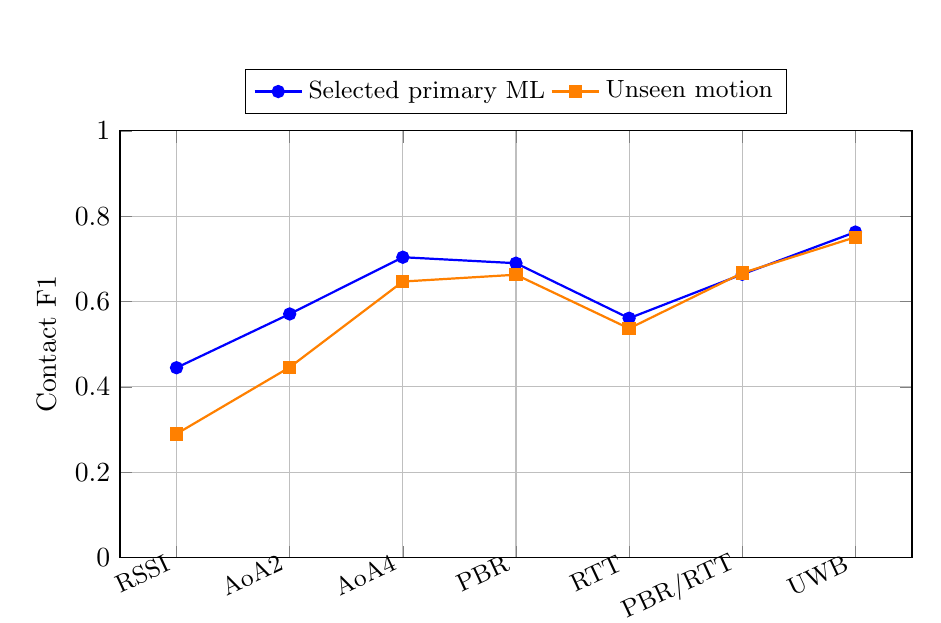
\begin{tikzpicture}\begin{axis}[width=.96\linewidth,height=7cm,xmin=.5,xmax=7.5,xtick={1,2,3,4,5,6,7},xticklabels={RSSI,AoA2,AoA4,PBR,RTT,PBR/RTT,UWB},xticklabel style={font=\small,rotate=25,anchor=east},grid=major,ylabel={Contact F1},ymin=0,ymax=1,legend style={font=\small,at={(.5,1.04)},anchor=south,legend columns=2}]
\addplot[blue,thick,mark=*] coordinates {(1,0.445) (2,0.571) (3,0.704) (4,0.69) (5,0.561) (6,0.664) (7,0.763)};\addlegendentry{Selected primary ML}
\addplot[orange,thick,mark=square*] coordinates {(1,0.29) (2,0.446) (3,0.647) (4,0.663) (5,0.537) (6,0.667) (7,0.751)};\addlegendentry{Unseen motion}
\end{axis}\end{tikzpicture}
\caption{Selected primary and unseen-motion F1 on the same map}\label{fig:generalization}
\end{figure}


The ideal setting is named LOS in artifact identifiers but does not guarantee that every two-room link has physical line of sight. Every selected method has lower primary F1 in the wall setting. The unfamiliar movement challenge retains the same map and radio assumptions; it is not a separate hospital, hardware, or participant evaluation.

\section{Contact Session Reconstruction Results}
Table~\ref{tab:primary} reports models selected exclusively using validation. The selected boosted-tree RSSI detector attains mean contact F1 0.445, compared with zero for the tuned geometric rule. Two and four angular receivers increase selected-model F1 to 0.571 and 0.704. PBR, RTT and PBR\_RTT attain 0.690, 0.561 and 0.664, respectively. UWB reaches 0.763 under the assumed UWB timing/bias and service conditions.

\begingroup
\small\setstretch{1.05}\setlength{\tabcolsep}{3pt}
\begin{longtable}{>{\raggedright\arraybackslash}p{0.147\linewidth}>{\raggedright\arraybackslash}p{0.147\linewidth}>{\raggedright\arraybackslash}p{0.147\linewidth}>{\raggedright\arraybackslash}p{0.147\linewidth}>{\raggedright\arraybackslash}p{0.147\linewidth}>{\raggedright\arraybackslash}p{0.147\linewidth}}
\caption{Validation-selected primary contact reconstruction}\label{tab:primary}\\
\toprule
\textbf{Budget} & \textbf{Family} & \textbf{Rule F1} & \textbf{ML F1} & \textbf{TP/FP/FN} & \textbf{ML minus rule 95\% interval}\\
\midrule
\endfirsthead
\toprule
\textbf{Budget} & \textbf{Family} & \textbf{Rule F1} & \textbf{ML F1} & \textbf{TP/FP/FN} & \textbf{ML minus rule 95\% interval}\\
\midrule
\endhead
\bottomrule
\endfoot
RSSI & Boosted & 0.000 & 0.445 & 217/\allowbreak{}464/\allowbreak{}135 & 0.445 [0.403, 0.488]\\
Ao\allowbreak{}A2 & Forest & 0.392 & 0.571 & 232/\allowbreak{}262/\allowbreak{}120 & 0.179 [0.122, 0.236]\\
Ao\allowbreak{}A4 & Forest & 0.579 & 0.704 & 285/\allowbreak{}196/\allowbreak{}67 & 0.125 [0.083, 0.171]\\
PBR & Boosted & 0.575 & 0.690 & 250/\allowbreak{}114/\allowbreak{}102 & 0.115 [0.063, 0.168]\\
RTT & Logistic & 0.485 & 0.561 & 252/\allowbreak{}323/\allowbreak{}100 & 0.076 [0.020, 0.128]\\
PBR/\allowbreak{}RTT & Boosted & 0.547 & 0.664 & 237/\allowbreak{}112/\allowbreak{}115 & 0.117 [0.060, 0.172]\\
UWB & Logistic & 0.729 & 0.763 & 261/\allowbreak{}90/\allowbreak{}91 & 0.034 [-0.009, 0.082]\\
\end{longtable}
\endgroup


Note: TP/FP/FN are pooled session counts across the primary test recordings and both matched sensor conditions. F1 is averaged across supported conditions within each seed and then across seeds; the interval concerns the paired seed-level ML-minus-rule F1 difference. Consequently, F1 calculated directly from these pooled counts is a different aggregation and will not generally equal the reported F1.

The improvement is not equivalent to sufficient reliability. RSSI produces 217 true positives, 464 false positives and 135 false negatives when the matched test conditions are pooled. Four-angle inference produces 285/196/67, and UWB 261/90/91. All configurations miss valid sessions and create false ones. These counts duplicate each underlying motion reference under two sensor settings and should not be interpreted as independent patient encounters.

The selected four-angle forest remains the primary method although boosted trees attain slightly higher final F1. Likewise, the selected RTT logistic model is not replaced by the better-scoring final forest. Table~\ref{tab:families} exposes all families and controls rather than presenting only whichever test model ranks first.

\begingroup
\small\setstretch{1.05}\setlength{\tabcolsep}{3pt}
\begin{longtable}{>{\raggedright\arraybackslash}p{0.110\linewidth}>{\raggedright\arraybackslash}p{0.110\linewidth}>{\raggedright\arraybackslash}p{0.110\linewidth}>{\raggedright\arraybackslash}p{0.110\linewidth}>{\raggedright\arraybackslash}p{0.110\linewidth}>{\raggedright\arraybackslash}p{0.110\linewidth}>{\raggedright\arraybackslash}p{0.110\linewidth}>{\raggedright\arraybackslash}p{0.110\linewidth}}
\caption{Primary contact F1 across full families and controls}\label{tab:families}\\
\toprule
\textbf{Budget} & \textbf{Strict} & \textbf{Temporal} & \textbf{Tuned} & \textbf{Logistic} & \textbf{Forest} & \textbf{Boosted} & \textbf{Bayes}\\
\midrule
\endfirsthead
\toprule
\textbf{Budget} & \textbf{Strict} & \textbf{Temporal} & \textbf{Tuned} & \textbf{Logistic} & \textbf{Forest} & \textbf{Boosted} & \textbf{Bayes}\\
\midrule
\endhead
\bottomrule
\endfoot
RSSI & 0.000 & 0.000 & 0.000 & 0.372 & 0.395 & 0.445 & 0.311\\
Ao\allowbreak{}A2 & 0.008 & 0.063 & 0.392 & 0.508 & 0.571 & 0.564 & 0.461\\
Ao\allowbreak{}A4 & 0.272 & 0.429 & 0.579 & 0.691 & 0.704 & 0.708 & 0.581\\
PBR & 0.450 & 0.520 & 0.575 & 0.667 & 0.651 & 0.690 & 0.664\\
RTT & 0.018 & 0.074 & 0.485 & 0.561 & 0.590 & 0.578 & 0.522\\
PBR/\allowbreak{}RTT & 0.439 & 0.504 & 0.547 & 0.658 & 0.649 & 0.664 & 0.660\\
UWB & 0.644 & 0.742 & 0.729 & 0.763 & 0.760 & 0.751 & 0.709\\
\end{longtable}
\endgroup


The selected model's pointwise paired interval lies above zero for RSSI, both angular budgets, PBR, RTT and PBR\_RTT. For UWB the mean difference is only 0.034 and the interval spans -0.009 to 0.082. Its higher absolute contact F1 therefore does not establish a clear incremental ML benefit over its equally tuned rule. The fixed 2 m temporal UWB rule also performs well, with mean F1 0.742. Figure~\ref{fig:paired-effects} presents the paired effects; the intervals are not simultaneous significance guarantees.


\begin{figure}[htbp]
\centering
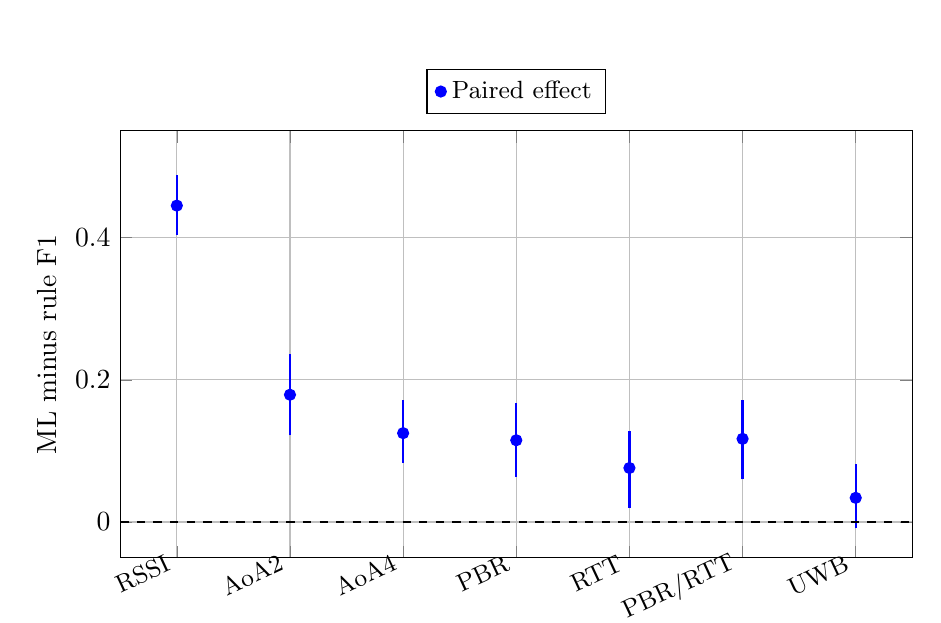
\begin{tikzpicture}\begin{axis}[width=.96\linewidth,height=7cm,xmin=.5,xmax=7.5,xtick={1,2,3,4,5,6,7},xticklabels={RSSI,AoA2,AoA4,PBR,RTT,PBR/RTT,UWB},xticklabel style={font=\small,rotate=25,anchor=east},grid=major,ylabel={ML minus rule F1},ymin=-.05,ymax=.55,legend style={font=\small,at={(.5,1.04)},anchor=south,legend columns=2}]
\addplot[only marks,mark=*,blue] coordinates {(1,0.445) (2,0.179) (3,0.125) (4,0.115) (5,0.076) (6,0.117) (7,0.034)};\addlegendentry{Paired effect}
\addplot[blue,thick,forget plot] coordinates {(1,0.403) (1,0.488)};
\addplot[blue,thick,forget plot] coordinates {(2,0.122) (2,0.236)};
\addplot[blue,thick,forget plot] coordinates {(3,0.083) (3,0.171)};
\addplot[blue,thick,forget plot] coordinates {(4,0.063) (4,0.168)};
\addplot[blue,thick,forget plot] coordinates {(5,0.02) (5,0.128)};
\addplot[blue,thick,forget plot] coordinates {(6,0.06) (6,0.172)};
\addplot[blue,thick,forget plot] coordinates {(7,-0.009) (7,0.082)};
\addplot[dashed,black,forget plot] coordinates {(.5,0)(7.5,0)};\end{axis}\end{tikzpicture}
\caption{Exploratory paired selected-ML minus tuned-rule F1 intervals}\label{fig:paired-effects}
\end{figure}


The learned Markov extension yields lower primary contact F1 than the corresponding selected full classifier in all seven configurations. For RSSI the scores are 0.378 versus 0.445; for four angles, 0.660 versus 0.704; and for UWB, 0.707 versus 0.763. Additional temporal modeling therefore does not automatically improve this pipeline. Correlated feature histories, the approximate emission formulation and validation-selected decoding are plausible contributors, but this experiment does not isolate their causal roles.

\begingroup
\small\setstretch{1.05}\setlength{\tabcolsep}{3pt}
\begin{longtable}{>{\raggedright\arraybackslash}p{0.188\linewidth}>{\raggedright\arraybackslash}p{0.188\linewidth}>{\raggedright\arraybackslash}p{0.188\linewidth}>{\raggedright\arraybackslash}p{0.188\linewidth}>{\raggedright\arraybackslash}p{0.188\linewidth}}
\caption{Primary contact F1 for temporal extension and ablations}\label{tab:ablations}\\
\toprule
\textbf{Budget} & \textbf{Selected full} & \textbf{Markov} & \textbf{No history} & \textbf{No room feature}\\
\midrule
\endfirsthead
\toprule
\textbf{Budget} & \textbf{Selected full} & \textbf{Markov} & \textbf{No history} & \textbf{No room feature}\\
\midrule
\endhead
\bottomrule
\endfoot
RSSI & 0.445 & 0.378 & 0.279 & 0.365\\
Ao\allowbreak{}A2 & 0.571 & 0.495 & 0.524 & 0.517\\
Ao\allowbreak{}A4 & 0.704 & 0.660 & 0.629 & 0.657\\
PBR & 0.690 & 0.640 & 0.663 & 0.686\\
RTT & 0.561 & 0.485 & 0.545 & 0.512\\
PBR/\allowbreak{}RTT & 0.664 & 0.651 & 0.656 & 0.683\\
UWB & 0.763 & 0.707 & 0.769 & 0.754\\
\end{longtable}
\endgroup


Removing contact history lowers RSSI F1 to 0.279 and four-angle F1 to 0.629. In contrast, the UWB history ablation attains 0.769, slightly above the full model's 0.763. Removing the room feature lowers several configurations but raises PBR\_RTT F1 from 0.664 to 0.683. These observations argue against claiming universal benefits for every feature group. Since ablations are refitted and receive independent validation-selected decisions, their effects include fitting and decoding interactions, not a simple feature deletion from one fixed predictor.

The PBR/RTT gate does not improve selected primary F1 over PBR alone. Both raw mechanisms and resulting feature distributions differ, and the models are fitted separately. This comparison demonstrates no benefit under the implemented gate and assumptions; it is not a rejection of standards-based cross-checking or better fusion estimators.

\begingroup
\small\setstretch{1.05}\setlength{\tabcolsep}{3pt}
\begin{longtable}{>{\raggedright\arraybackslash}p{0.188\linewidth}>{\raggedright\arraybackslash}p{0.188\linewidth}>{\raggedright\arraybackslash}p{0.188\linewidth}>{\raggedright\arraybackslash}p{0.188\linewidth}>{\raggedright\arraybackslash}p{0.188\linewidth}}
\caption{Table C1 Frozen primary model and rule settings}\label{tab:selections}\\
\toprule
\textbf{Budget} & \textbf{Family} & \textbf{Hyperparameter} & \textbf{ML threshold / decoder} & \textbf{Rule distance / decoder}\\
\midrule
\endfirsthead
\toprule
\textbf{Budget} & \textbf{Family} & \textbf{Hyperparameter} & \textbf{ML threshold / decoder} & \textbf{Rule distance / decoder}\\
\midrule
\endhead
\bottomrule
\endfoot
RSSI & Boosted & leaves=31 & 0.2 /\allowbreak{} occupancy & 2 m /\allowbreak{} strict\\
Ao\allowbreak{}A2 & Forest & depth=12 & 0.2 /\allowbreak{} strict & 3 m /\allowbreak{} occupancy\\
Ao\allowbreak{}A4 & Forest & depth=8 & 0.2 /\allowbreak{} strict & 3 m /\allowbreak{} strict\\
PBR & Boosted & leaves=15 & 0.2 /\allowbreak{} strict & 3 m /\allowbreak{} occupancy\\
RTT & Logistic & C=1.0 & 0.2 /\allowbreak{} occupancy & 3 m /\allowbreak{} occupancy\\
PBR/\allowbreak{}RTT & Boosted & leaves=15 & 0.2 /\allowbreak{} strict & 3 m /\allowbreak{} occupancy\\
UWB & Logistic & C=1.0 & 0.2 /\allowbreak{} strict & 2.5 m /\allowbreak{} strict\\
\end{longtable}
\endgroup


\section{Probabilistic Exposure Risk Assessment}
Table~\ref{tab:quality} reports instantaneous probability diagnostics together with contact-time and false-session outcomes. The prior-only mean Brier score is 0.077 for every modality. Selected-model Brier values range from 0.024 for UWB to 0.064 for RSSI. ECE ranges from 0.012 to 0.038. These improvements over a prevalence baseline do not establish session-level calibration, especially because per-frame class imbalance and temporal dependence remain substantial.

\begingroup
\small\setstretch{1.05}\setlength{\tabcolsep}{3pt}
\begin{longtable}{>{\raggedright\arraybackslash}p{0.126\linewidth}>{\raggedright\arraybackslash}p{0.126\linewidth}>{\raggedright\arraybackslash}p{0.126\linewidth}>{\raggedright\arraybackslash}p{0.126\linewidth}>{\raggedright\arraybackslash}p{0.126\linewidth}>{\raggedright\arraybackslash}p{0.126\linewidth}>{\raggedright\arraybackslash}p{0.126\linewidth}}
\caption{Selected-model probability and time outcomes}\label{tab:quality}\\
\toprule
\textbf{Budget} & \textbf{Brier} & \textbf{ECE} & \textbf{Missed time rate} & \textbf{FP per pair-hour} & \textbf{Duration MAE s} & \textbf{Confirm delay s}\\
\midrule
\endfirsthead
\toprule
\textbf{Budget} & \textbf{Brier} & \textbf{ECE} & \textbf{Missed time rate} & \textbf{FP per pair-hour} & \textbf{Duration MAE s} & \textbf{Confirm delay s}\\
\midrule
\endhead
\bottomrule
\endfoot
RSSI & 0.064 & 0.038 & 0.442 & 2.762 & 54.0 & 37.7\\
Ao\allowbreak{}A2 & 0.049 & 0.022 & 0.407 & 1.560 & 34.9 & 40.2\\
Ao\allowbreak{}A4 & 0.033 & 0.015 & 0.241 & 1.167 & 33.6 & 41.5\\
PBR & 0.029 & 0.012 & 0.359 & 0.679 & 35.0 & 41.1\\
RTT & 0.046 & 0.018 & 0.377 & 1.923 & 43.9 & 43.3\\
PBR/\allowbreak{}RTT & 0.029 & 0.013 & 0.399 & 0.667 & 34.4 & 40.8\\
UWB & 0.024 & 0.013 & 0.263 & 0.536 & 30.4 & 37.8\\
\end{longtable}
\endgroup


RSSI misses 44.2\% of qualified reference pair-time and produces 2.762 false sessions per pair-hour. Four-angle inference misses 24.1\%, and UWB misses 26.3\%, despite UWB's higher event F1. Thus event ranking and interval coverage need not agree. The mean conditional duration errors are about 54.0 s, 33.6 s and 30.4 s for these three configurations. Their average per-recording median confirmation delays are about 37.7 s, 41.5 s and 37.8 s. Missing sessions are absent from these conditional delay/error summaries, which should not be interpreted as an end-to-end reliability guarantee.

Probability reliability is summarized by the retained Brier/ECE table. The original scientific plots remain in the research artifacts; no infection-calibration inference is drawn from them.

The section title is retained from the supplied report, but these are probability-quality metrics for instantaneous proximity, not calibrated MDR-TB exposure or infection. The prior-only Brier baseline is 0.077. All selected models improve on it, yet session false alarms and missed time remain substantial.

A frame can be predicted well while a long event is fragmented. Conversely, an event can match under permissive overlap tolerance while its boundaries are wrong. The probability and session tables must therefore be interpreted together.

\section{Edge Processing and Scalability Results}
A separate ranging campaign used 30 seeds, eight scored moving tags, three scheduled-client loads, and six methods. Additional 32/128-client settings introduced background service demand without adding physical crowd trajectories. Table~\ref{tab:service} shows the UWB branch as an illustrative scheduling comparison. Active-ranging event F1 collapsed at higher loads for all ranging branches under four slots per second and the three-second estimate-expiry rule. The passive branches repeated unchanged across those loads by design.

\begingroup
\small\setstretch{1.05}\setlength{\tabcolsep}{3pt}
\begin{longtable}{>{\raggedright\arraybackslash}p{0.235\linewidth}>{\raggedright\arraybackslash}p{0.235\linewidth}>{\raggedright\arraybackslash}p{0.235\linewidth}>{\raggedright\arraybackslash}p{0.235\linewidth}}
\caption{Separate UWB service-load study}\label{tab:service}\\
\toprule
\textbf{Channel setting} & \textbf{Scheduled clients} & \textbf{Mean contact F1} & \textbf{Availability}\\
\midrule
\endfirsthead
\toprule
\textbf{Channel setting} & \textbf{Scheduled clients} & \textbf{Mean contact F1} & \textbf{Availability}\\
\midrule
\endhead
\bottomrule
\endfoot
LOS & 8 & 0.938 & 0.995\\
LOS & 32 & 0.000 & 0.472\\
LOS & 128 & 0.000 & 0.127\\
wall-multipath & 8 & 0.783 & 0.977\\
wall-multipath & 32 & 0.000 & 0.443\\
wall-multipath & 128 & 0.000 & 0.119\\
\end{longtable}
\endgroup


This outcome demonstrates that an imposed low update budget can prevent temporal reconstruction even when available range estimates are comparatively accurate. It does not identify the maximum capacity of BLE Channel Sounding or UWB, and it does not predict performance of optimized device scheduling or UWB TDoA. Procedure-specific airtime, concurrent measurements and energy accounting require additional modeling or measurements. The v7 learned detectors were not trained or evaluated on these higher-load settings.

A practical cost comparison must account for complete wearables and infrastructure. We express deployment cost symbolically as

\begin{equation}
\begin{aligned}C_{\mathrm{total}}={}&NC_{\mathrm{tag}}+AC_{\mathrm{anchor}}+C_{\mathrm{backhaul}}\\&+C_{\mathrm{calibration}}+C_{\mathrm{spares}}+C_{\mathrm{operations}}+C_{\mathrm{maintenance}}\end{aligned}
\label{eq:source11}
\end{equation}

Here N is the wearable count and A the installed gateway/anchor count. Tag cost includes radio/processor, antenna, board, power system, enclosure, assembly, provisioning and product validation. Infrastructure cost includes installation and the appropriate receiver capabilities. Reusable hospital deployments also involve charging, cleaning, replacement and handling labor. No term was measured in this study, and the equation does not establish a minimum-cost configuration.

RSSI-only observations minimize added sensing capabilities in the benchmark but currently produce a high false-contact burden. Angular receivers require compatible direction-finding tags and receiver arrays. PBR/RTT requires compatible channel-sounding radios; compatibility cannot be inferred from generic BLE support. UWB introduces its own compatible radio and infrastructure requirements, although integrated UWB/BLE modules exist \cite{ref12}. A higher tag cost can sometimes be offset by lower infrastructure or operational costs; only comparable complete-system quotations can test that hypothesis.

The present results therefore support retaining UWB as a comparator rather than discarding it on an assumed cost basis. They also support studying lower-cost integrated ranging options and observation-triggered scheduling. They do not support declaring BLE always cheaper, UWB always more accurate, or a hybrid rollout adequate for devices that lack the required measurements. Energy, capacity, accuracy and operational burden must be assessed together in a hardware-informed follow-up.

\section{Privacy Evaluation Results}
The main v7 experiment does not provide a numerical anonymity, encryption-strength, or re-identification-resistance result. Its privacy-relevant architectural property is predictor minimization: true identity, source clinical status, seed, time as a predictor, and hidden geometry are excluded from X. Synthetic identifiers remain necessary to maintain histories and outputs.

The retained historical privacy code studies different attacker interfaces and rotation behavior under its own protocols. Its outcomes must remain attached to those settings; they cannot be transferred to the final classifier comparison as a security certificate. This report therefore replaces the old template's unspecified privacy percentages with an explicit evidence-status table.

\begingroup
\small\setstretch{1.05}\setlength{\tabcolsep}{3pt}
\begin{longtable}{>{\raggedright\arraybackslash}p{0.200\linewidth}>{\raggedright\arraybackslash}p{0.400\linewidth}>{\raggedright\arraybackslash}p{0.340\linewidth}}
\caption{Privacy evidence boundaries}\label{tab:privacy}\\
\toprule
\textbf{Property} & \textbf{Current evidence} & \textbf{Not established}\\
\midrule
\endfirsthead
\toprule
\textbf{Property} & \textbf{Current evidence} & \textbf{Not established}\\
\midrule
\endhead
\bottomrule
\endfoot
Predictor minimization & Identity/\allowbreak{}clinical status/\allowbreak{}hidden truth excluded from v7 X & Anonymity of a deployed system\\
Pseudonym generation & HMAC and simulation-grade modes in historical source & Production key-management security\\
Authorized resolution & Registry interface with authorization context & Audited authenticated hospital service\\
Linkability evaluation & Historical attacker-model modules retained & Resistance to all re-identification\\
Joint rotation/\allowbreak{}contact inference & Not part of final learned benchmark & Utility under real rotating devices\\
\end{longtable}
\endgroup


A complete deployment assessment would examine authenticated identity resolution, registry compromise, behavioral linkability, radio metadata, access logging, and key management. It would also evaluate whether rotation fragments the histories required by the learned detector.

\section{System Output and Dashboard}
Authoritative outputs are probability arrays, decoded decisions, predicted session records, per-case metrics, grouped summaries, paired contrasts, and manifests. A session record identifies a synthetic pair and includes start, end, and detectedAt. The detector's threshold and policy are stored with the bundle.

The retained React interface is a separate demonstration. The following screenshots were captured from the existing built application on 6 October 2026. Displayed names and statuses are synthetic. Interface labels such as infection probability, clinical surveillance, bandwidth saved, and gateway CPU/RAM are demonstration terminology or counters, not clinically calibrated outputs or benchmark measurements. The interface's larger population and hospital map are different from the eight-tag research fixture.


\begin{figure}[htbp]
\centering
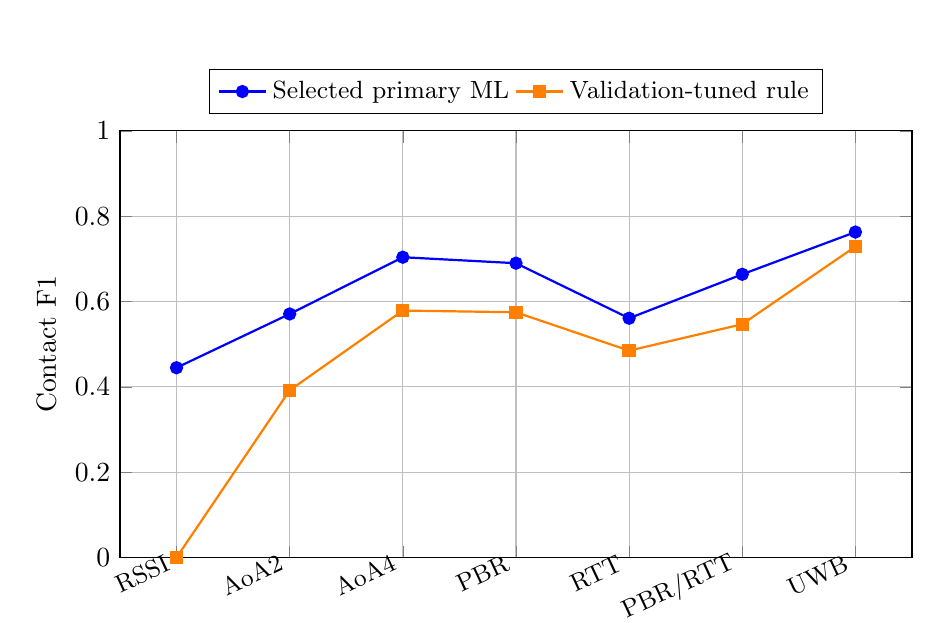
\begin{tikzpicture}\begin{axis}[width=.96\linewidth,height=7cm,xmin=.5,xmax=7.5,xtick={1,2,3,4,5,6,7},xticklabels={RSSI,AoA2,AoA4,PBR,RTT,PBR/RTT,UWB},xticklabel style={font=\small,rotate=25,anchor=east},grid=major,ylabel={Contact F1},ymin=0,ymax=1,legend style={font=\small,at={(.5,1.04)},anchor=south,legend columns=2}]
\addplot[blue,thick,mark=*] coordinates {(1,0.445) (2,0.571) (3,0.704) (4,0.69) (5,0.561) (6,0.664) (7,0.763)};\addlegendentry{Selected primary ML}
\addplot[orange,thick,mark=square*] coordinates {(1,0) (2,0.392) (3,0.579) (4,0.575) (5,0.485) (6,0.547) (7,0.729)};\addlegendentry{Validation-tuned rule}
\end{axis}\end{tikzpicture}
\caption{Research-output view of frozen aggregate outcomes; not an application screenshot}\label{fig:output}
\end{figure}


A reviewer should consult results/ml-v7-models-complete for fitted selections, results/ml-v7-evaluation for outcomes, and results/ml-v7-report for readable tables. The interrupted results/ml-v7-models directory is retained but nonauthoritative. Displayed old risk heuristics must not replace these artifacts.

\begin{figure}[p]\centering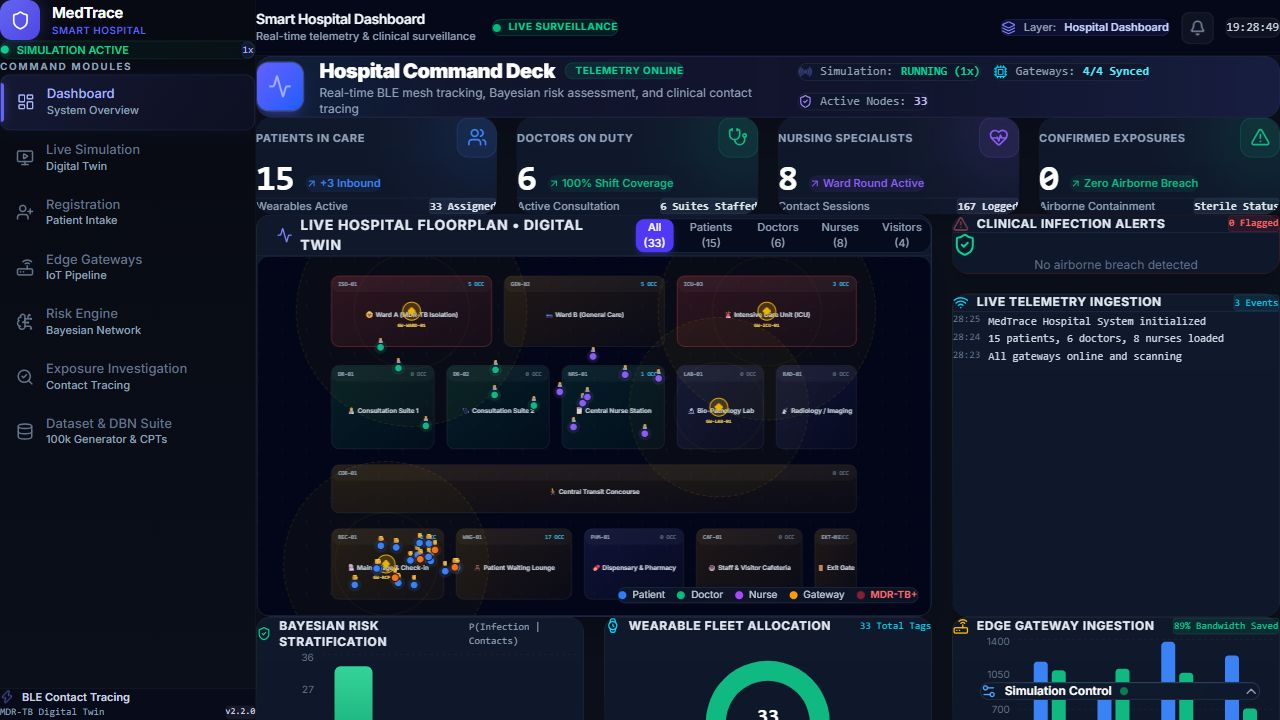
\includegraphics[width=\linewidth,height=.74\textheight,keepaspectratio]{dashboard.jpg}\caption{Actual dashboard demonstration. Displayed clinical and performance labels are not verified research outcomes.}\label{fig:screen-dashboard}\end{figure}

\begin{figure}[p]\centering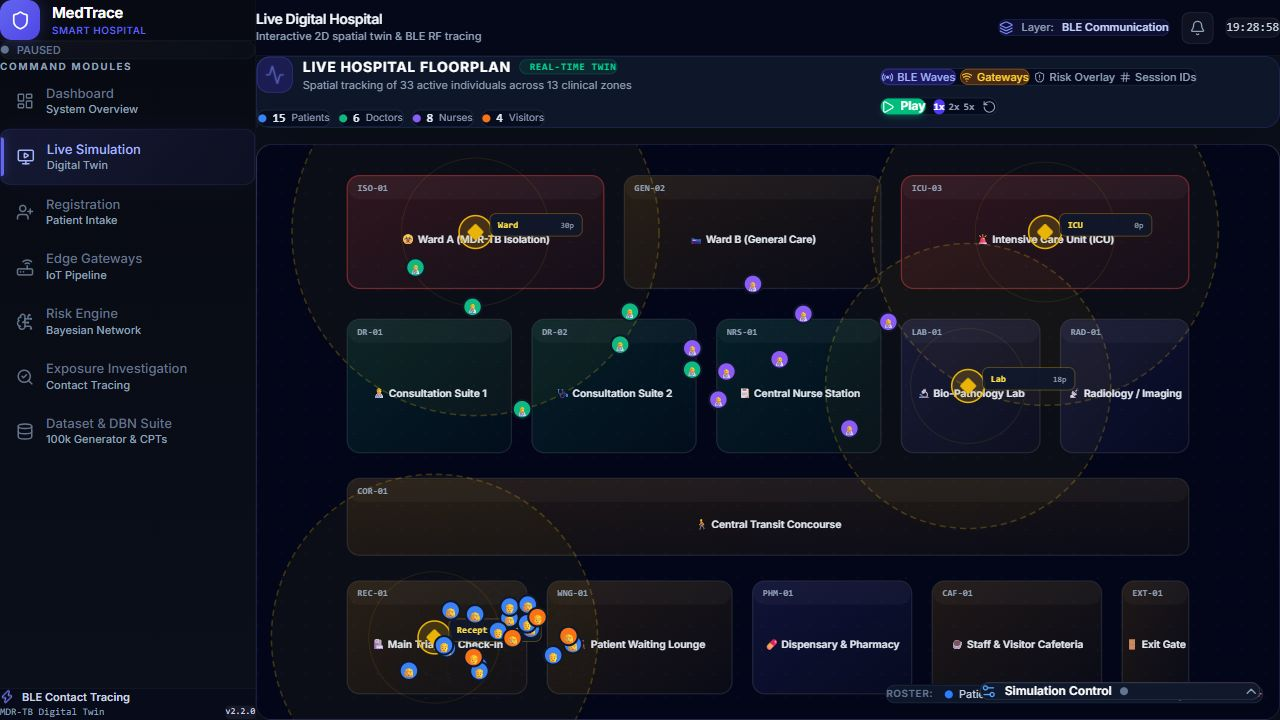
\includegraphics[width=\linewidth,height=.74\textheight,keepaspectratio]{live-simulation.jpg}\caption{Actual paused live-simulation interface; its synthetic hospital scene differs from the v7 two-room fixture.}\label{fig:screen-live-simulation}\end{figure}

\begin{figure}[p]\centering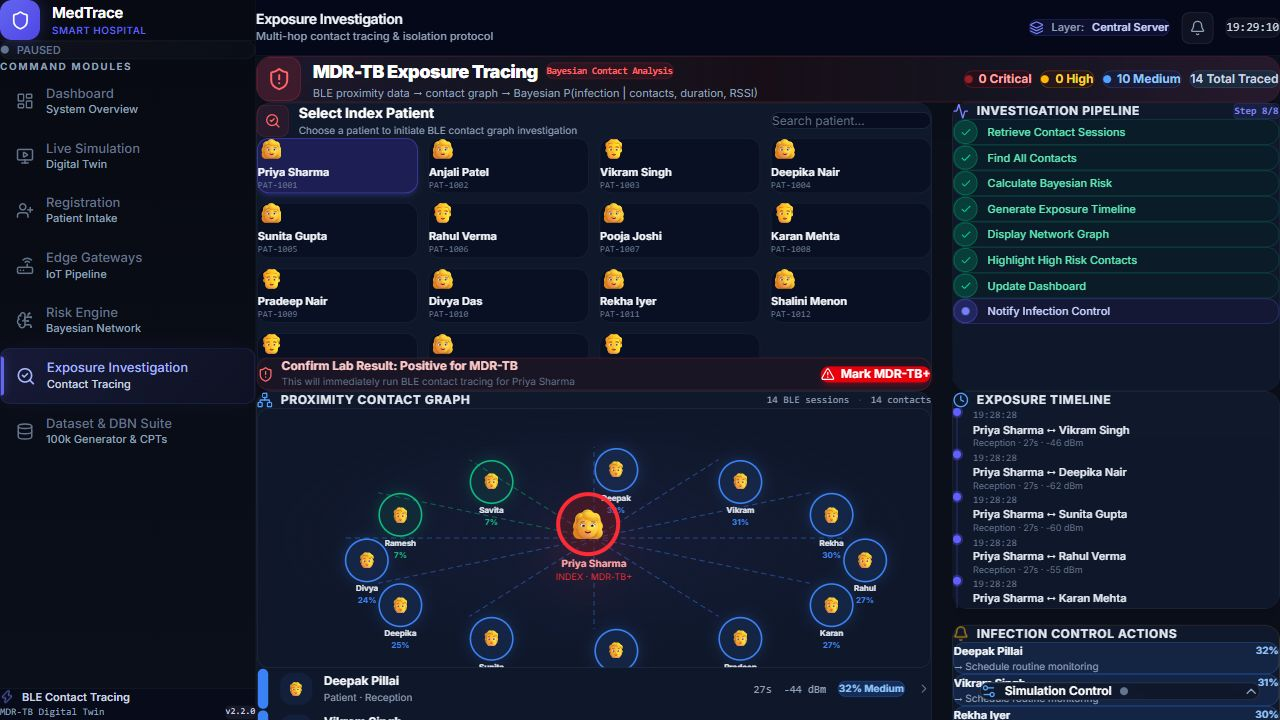
\includegraphics[width=\linewidth,height=.74\textheight,keepaspectratio]{contact-investigation.jpg}\caption{Actual contact-investigation interface with synthetic records; no clinical action or diagnosis was performed.}\label{fig:screen-contact-investigation}\end{figure}

\begin{figure}[p]\centering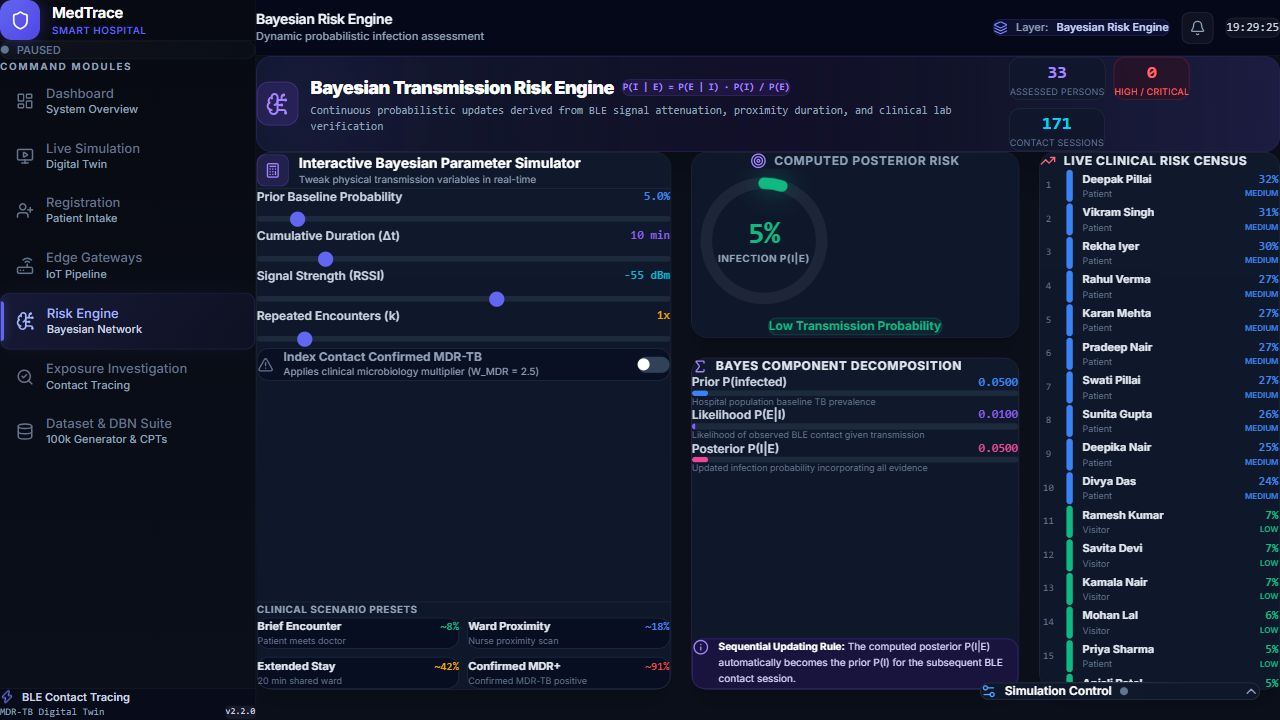
\includegraphics[width=\linewidth,height=.74\textheight,keepaspectratio]{risk-demonstration.jpg}\caption{Actual historical risk-engine interface. Displayed infection probabilities are heuristic demonstration values, not clinically validated probabilities.}\label{fig:screen-risk-demonstration}\end{figure}

\begin{figure}[p]\centering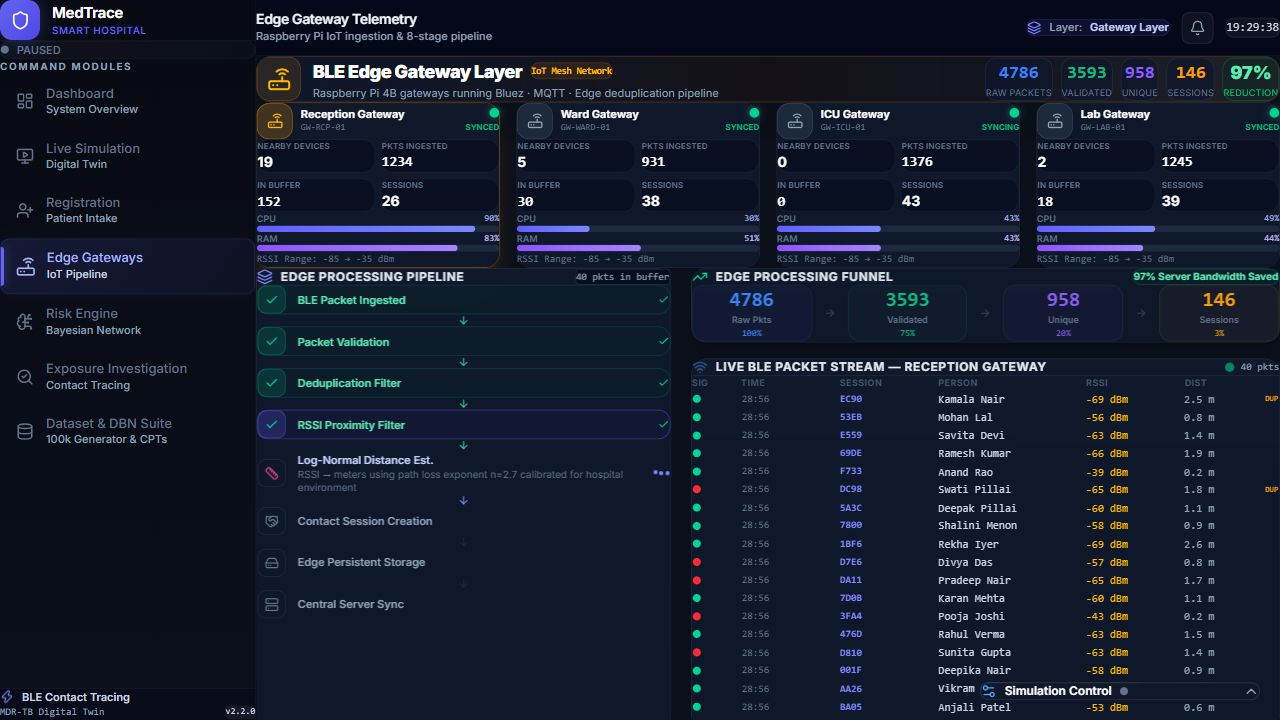
\includegraphics[width=\linewidth,height=.74\textheight,keepaspectratio]{gateway.jpg}\caption{Actual gateway interface. Its hardware, bandwidth, CPU/RAM, and packet counters are demonstration displays, not measured hospital deployment evidence.}\label{fig:screen-gateway}\end{figure}

\section{Discussion}
Learned decisions combine noisy estimates with signal agreement and causal history, recovering sustained contacts that strict geometry can miss. The strongest RSSI relative improvement occurs against a comparator that reconstructs no qualified sessions, so its magnitude should be read with absolute error counts. Additional angular/ranging observations improve the selected-model event scores under the declared assumptions, but the improvement depends on map, trajectories, covariance choices and error distributions.

The best full family differs across modalities. This is compatible with different feature/error structures, but the small validation population and finite candidate grids also contribute to selection variability. We deliberately retain test underperformance relative to other families rather than selecting test winners. A neural sequence model, learned localization network or more elaborate ranging fusion could be investigated, but this dataset does not establish that added model complexity would help, and no such unimplemented model is credited in the results.

Same-room 2 m proximity for 30 elapsed seconds is an operational simulation target. It excludes contacts across a wall and does not represent ventilation, pathogens, susceptibility, protective equipment, face orientation or exposure dose. The one-second sampling cannot guarantee continuous physical proximity between samples. Treating geometric contacts as infection events would change the construct and require independent clinical evidence.

The radio models use assumed Gaussian noise, link/device biases and a simplified wall intersection. The reciprocal two-path PBR channel, ideal timing intervals and common BLE reception mask omit real antenna patterns, device orientation dynamics, frequency-dependent calibration, hardware timestamp errors, body geometry, interference and radio stack behavior. Nominal error parameters are neither measured technology specifications nor vendor guarantees. Conclusions about relative technology performance are conditional on these assumptions.

Seed-grouped partitions, frozen selection, current-time features and modality stripping reduce several leakage risks. Independent arithmetic and geometry checks establish consistency of the saved evidence; they do not prove the simulator itself is a faithful physical model. The public map supplies useful information, and removing one room indicator does not remove all map-related effects. Missing-estimate gating changes the attainable recall and the frame probability distribution.

Temporal matching tolerances are fixed and permissive, and greedy matching may differ from optimal assignment in complex overlapping predictions. Conditional duration and delay omit misses. F1 does not capture every operational tradeoff; false sessions and missed contact time may dominate a real monitoring workflow. Sensitivity to matching tolerance, time step, map layout and decision penalties is not quantified by the present main experiment.

The primary study has 30 independent test motion seeds, and only eight validation and calibration seeds. Frame counts do not provide independent sample size. Both sensor settings repeat each motion, and bootstrap intervals cover within-simulator seed variability only. Pointwise comparisons across seven modalities and multiple ablations lack multiplicity adjustment; exploratory positive intervals are not confirmatory clinical hypothesis tests. Calibration curves pool correlated observations and should not be interpreted as independent-frame confidence evidence.

All main experiments use eight moving tags and one map. Independent waypoints change the motion family but not hospital, hardware, location, channel assumptions or participant population. The service-load study adds virtual traffic rather than crowds. The trajectories are deliberately constructed research scenarios, not measured staffing, patient, visitor or workflow distributions. Generalizing them to a dense hospital needs separately designed maps, populations and movement patterns.

A practical next study would collect labeled distance/contact sequences with independent people, devices, locations or days, fit channel and calibration parameters using development recordings, and freeze inference before evaluating untouched recordings. It should include wall barriers, short encounters, orientation changes, missing packets and sustained contacts, while measuring radio update rate, procedure duration, wearable power and comparable complete-system cost. Such data would test whether the observed learning gains survive model mismatch; that empirical question remains open.

The corrected original campaign used 50 people, eight gateways and 30 seeds under a different simulation protocol. It reconstructed 161 sessions against 84 reference sessions, with TP = 3, FP = 158 and FN = 81. Pooled precision is 3/161 = 1.86\% and pooled recall is 3/84 = 3.57\%; these differ from its seed-mean metrics. This negative result motivates evaluating inference before relying on surviving candidate records for learning. It is not a baseline rerun on the present eight-tag recordings and cannot be pooled with Table~\ref{tab:primary}.

The original downstream task contained 322 directed records but only six positive directions, corresponding to three distinct matched sessions. A corrected accessor and temporal-label path produced newly versioned outputs; the fixed likelihood-table Bayesian score in that campaign is distinct from our learned Gaussian Bayes and Markov models. We retain this study as supporting provenance rather than using its sparse ranking outcomes to establish a general model hierarchy. The earlier unverified 811-FP diagnostic is not a result of this paper.

\chapter{PROJECT IMPACT AND SDG MAPPING}

\section{Project Impact}
The completed impact is a reproducible technical benchmark and an inspectable project architecture. Potential future hospital value depends on measured deployment validity and cannot be established from synthetic F1 alone. The following subsections distinguish completed research contributions from intended operational benefits.

\subsection{Improved Contact Monitoring}
The all-pair learned approach recovers synthetic sustained contacts that declared geometric rules can miss. Angular and ranging budgets improve several primary scores under matched assumptions. The study also exposes substantial false-session and missed-time burdens, preventing optimistic claims based on a single favorable score.

Potential hospital monitoring would require independently measured contact references, device and map calibration, and operational acceptance criteria. The current impact is evidence about an algorithmic comparison, not a demonstrated reduction in disease transmission.

\subsection{Reduced Data Transmission and Processing Load}
The original modular edge architecture supports validation, deduplication, filtering, and aggregation before forwarding data. These are reasonable ways to avoid redundant representations. However, no new measured communication-reduction or hospital throughput claim is established by the final study.

The separate load experiment shows how a restrictive update schedule can defeat sustained reconstruction. Future optimization must preserve useful observation availability rather than treating maximum compression as the sole objective.

\subsection{Privacy-Preserving Monitoring}
The companion identity architecture demonstrates separation between public pseudonyms and protected mappings. The main predictor also excludes personal identity and clinical source status. These design choices support information minimization but do not establish a complete privacy guarantee.

Real impact depends on properly managed identities, secrets, access, retention, and consent/governance requirements. The deterministic simulation generator cannot be used as a claim of cryptographic protection.

\subsection{Probabilistic Exposure Assessment}
The completed probabilistic contribution is calibrated instantaneous proximity estimation with separately measured Brier and ECE outcomes. Reporting these alongside sessions makes uncertainty more visible than a binary display alone.

The outputs must not be promoted to biological exposure or infection probabilities. A later exposure model would need separate targets, relevant environmental and clinical information, and independently held-out empirical validation.

\subsection{Support for Infection-Control Decision Making}
A validated future system could offer contact histories for human review as one source among institutional and clinical records. This project provides a technical foundation for studying whether such histories can be recovered reliably.

Its current false-contact burden and limited external validity mean it is not ready to automate infection-control actions. Decisions should not be justified by translating the synthetic classifier's score into a clinical risk category.

\subsection{Research and Technological Impact}
The source, protocol, manuscript, and retained evidence are publicly inspectable. The release includes all 3,809 result files in 16 archives, with archive and member checksums. Saved-artifact verification independently checks 826,560 physical labels and 6,468 detector evaluations.

Negative evidence remains identifiable: the original gateway reconstruction performed poorly, the learned Markov extension lowered primary F1 in every modality, and the PBR/RTT gate did not improve the main PBR comparison. Preserving these outcomes improves the project's research value.

The contribution can support hardware-informed follow-up studies. It does not claim all algorithms were trained or that the software has been fully validated for hospital deployment.

\section{Mapped SDGs}
The United Nations defines SDG 3 around health and well-being, SDG 9 around infrastructure and innovation, and SDG 16 around accountable institutions \cite{ref18}. The mapping below is a statement of possible research alignment, not a measured contribution to a national indicator.

\begingroup
\small\setstretch{1.05}\setlength{\tabcolsep}{3pt}
\begin{longtable}{>{\raggedright\arraybackslash}p{0.200\linewidth}>{\raggedright\arraybackslash}p{0.400\linewidth}>{\raggedright\arraybackslash}p{0.340\linewidth}}
\caption{Project alignment with Sustainable Development Goals}\label{tab:sdg}\\
\toprule
\textbf{SDG} & \textbf{Goal} & \textbf{Research alignment and qualification}\\
\midrule
\endfirsthead
\toprule
\textbf{SDG} & \textbf{Goal} & \textbf{Research alignment and qualification}\\
\midrule
\endhead
\bottomrule
\endfoot
3 & Good Health and Well-Being & Potential foundation for contact-history research; no measured clinical impact.\\
9 & Industry, Innovation and Infrastructure & Reproducible sensing, estimation, and learning benchmark; no deployed infrastructure claim.\\
16 & Peace, Justice and Strong Institutions & Information-minimization and governance-oriented design; no complete privacy/\allowbreak{}security guarantee.\\
\end{longtable}
\endgroup


The project aligns most directly with reproducible sensing/inference research and responsible interpretation. Claims about health impact or institutional privacy must remain conditional on subsequent empirical validation. Unrelated cultural/dance material from the old template is excluded because it does not describe this project.

\chapter{CONCLUSION AND FUTURE SCOPE}

\section{Conclusion}
We evaluated sustained-contact reconstruction using seven matched observation budgets and four calibrated classifier families with causal features, grouped partitions and frozen model selection. The selected models improve mean event F1 relative to declared validation-tuned geometric comparators, with scores ranging from 0.445 for RSSI to 0.763 for UWB under the chosen synthetic assumptions. RSSI remains vulnerable to false contacts and unseen-motion degradation. UWB's incremental ML advantage is uncertain, and the learned Markov and PBR/RTT gate extensions provide no consistent primary improvement.

The findings support evaluating sensing, temporal contact inference and probability quality as separate components. They also show why localization accuracy, a large relative F1 gain or a low frame calibration error cannot alone establish a dependable low-cost hospital system. The resulting benchmark and retained evidence offer a reproducible foundation for hardware-informed contact research, while real deployment accuracy, cost, energy and clinical interpretation remain subjects for empirical validation.

The college project retains its original hospital-monitoring motivation and companion edge/privacy/dashboard modules, while the main experimental report now rests on the frozen trained contact comparison. Organizational cleanup, implementation checks, numerical reproduction, and scientific validity are separate achievements. Passing tests and compiling this report do not establish clinical effectiveness.

\section{Limitations}
Same-room 2 m proximity for 30 elapsed seconds is an operational simulation target. It excludes contacts across a wall and does not represent ventilation, pathogens, susceptibility, protective equipment, face orientation or exposure dose. The one-second sampling cannot guarantee continuous physical proximity between samples. Treating geometric contacts as infection events would change the construct and require independent clinical evidence.

The radio models use assumed Gaussian noise, link/device biases and a simplified wall intersection. The reciprocal two-path PBR channel, ideal timing intervals and common BLE reception mask omit real antenna patterns, device orientation dynamics, frequency-dependent calibration, hardware timestamp errors, body geometry, interference and radio stack behavior. Nominal error parameters are neither measured technology specifications nor vendor guarantees. Conclusions about relative technology performance are conditional on these assumptions.

Seed-grouped partitions, frozen selection, current-time features and modality stripping reduce several leakage risks. Independent arithmetic and geometry checks establish consistency of the saved evidence; they do not prove the simulator itself is a faithful physical model. The public map supplies useful information, and removing one room indicator does not remove all map-related effects. Missing-estimate gating changes the attainable recall and the frame probability distribution.

Temporal matching tolerances are fixed and permissive, and greedy matching may differ from optimal assignment in complex overlapping predictions. Conditional duration and delay omit misses. F1 does not capture every operational tradeoff; false sessions and missed contact time may dominate a real monitoring workflow. Sensitivity to matching tolerance, time step, map layout and decision penalties is not quantified by the present main experiment.

The primary study has 30 independent test motion seeds, and only eight validation and calibration seeds. Frame counts do not provide independent sample size. Both sensor settings repeat each motion, and bootstrap intervals cover within-simulator seed variability only. Pointwise comparisons across seven modalities and multiple ablations lack multiplicity adjustment; exploratory positive intervals are not confirmatory clinical hypothesis tests. Calibration curves pool correlated observations and should not be interpreted as independent-frame confidence evidence.

All main experiments use eight moving tags and one map. Independent waypoints change the motion family but not hospital, hardware, location, channel assumptions or participant population. The service-load study adds virtual traffic rather than crowds. The trajectories are deliberately constructed research scenarios, not measured staffing, patient, visitor or workflow distributions. Generalizing them to a dense hospital needs separately designed maps, populations and movement patterns.

A practical next study would collect labeled distance/contact sequences with independent people, devices, locations or days, fit channel and calibration parameters using development recordings, and freeze inference before evaluating untouched recordings. It should include wall barriers, short encounters, orientation changes, missing packets and sustained contacts, while measuring radio update rate, procedure duration, wearable power and comparable complete-system cost. Such data would test whether the observed learning gains survive model mismatch; that empirical question remains open.

\section{Future Scope}
Future work should test clear hypotheses rather than add advanced method names without evidence. The priorities below connect the simulator's limitations to measurable next steps. They are planned extensions, not already completed experiments.

\subsection*{Physical Hardware Implementation}
Collect synchronized radio observations from compatible BLE direction-finding/channel-sounding or UWB devices. Establish independent distance/contact references, measure device-specific biases, and validate timestamp units and phase conventions. Record wearable power, procedure duration, packet availability, and charging/cleaning requirements.

Do not substitute generic BLE compatibility for the capabilities required by AoA or PBR/RTT. Hardware selection must follow the implemented measurement needs and a comparable complete-system cost study.

\subsection*{Realistic Hospital Environment Testing}
Use independently designed maps, locations, movement routines, and participants after appropriate permissions. Separate people, devices, days, or sites across development and final test. Include walls, doorways, body orientation, near-threshold encounters, short visits, and missing packets.

Fit channel assumptions only on development measurements and freeze them before evaluating untouched recordings. Test whether the observed learning gains survive physical model mismatch.

\subsection*{Advanced Proximity Estimation}
Investigate improved range/angle fusion, bias-aware localization, measurement uncertainty, and resource-aware observation policies. A robust weighted fusion estimator differs from the current PBR/RTT consistency gate and must receive its own protocol and new results.

Sequence models or learned localization could be compared when sufficient independent data supports them. Current negative Markov findings show that extra temporal complexity is not automatically beneficial. Maintain strong tuned rules and publish ablation and adverse outcomes.

\subsection*{Enhanced Exposure-Risk Modelling}
Define an independently justified exposure construct before fitting a clinical or epidemiological model. Relevant information might include environmental conditions and protective measures, but must be collected, governed, and evaluated separately from geometric contact labels.

Do not relabel proximity probabilities as infection risk. Any such extension needs suitable outcomes, calibration, held-out validation, and ethical/institutional oversight.

\subsection*{Advanced Privacy and Security}
Evaluate contact continuity under rotating identifiers together with the learned pipeline. Replace simulation-only authorization assumptions with authenticated principals and secure registry/key management. Test behavioral linkage, compromise scenarios, transport security, access auditing, and retention controls.

Keep a declared threat model and report what each attack evaluation covers. Neither identifier rotation nor a single collision test establishes complete anonymity.

\subsection*{Large-Scale and Real-Time Deployment}
Extend beyond eight moving tags with physical crowd trajectories, multiple maps, and procedure-specific scheduling/airtime. Measure full sensing-to-server latency and resource use on intended hardware. Compare observation-triggered scheduling, parallel service, and alternative architectures without borrowing capacity claims from the current four-slot fixture.

Evaluate session quality at load alongside cost and battery consumption. The completed v7 comparison has not trained or tested the detectors on 32/128-client moving crowds.

\subsection*{Clinical and Epidemiological Validation}
Any study relating recorded contacts to biological outcomes requires independent clinical/epidemiological evidence and the relevant approvals. Geometric truth is useful for evaluating sensing but is not a clinical gold standard for infection.

A prospective study should preserve the separation between sensing validity, exposure interpretation, and outcome prediction. Real-world claims must specify participants, settings, uncertainty, and limitations rather than generalizing directly from synthetic seeds.

\subsection*{Integration with Hospital Information Systems}
A future integration could associate reviewed contact records with authorized institutional information through controlled interfaces. It would need role-based access, secure identity continuity, audit trails, clear retention rules, and a workflow for reviewing false alarms and missing evidence.

The completed reproducibility package is available at \url{https://github.com/ayyananwar/MDR-SIM}, with retained evidence in the research-v7-2026-10-06 release. A permanent archive DOI and author-agreed redistribution license have not yet been assigned. The source and report provide a foundation for further technical validation, not a ready clinical service.

\clearpage\pagestyle{plain}
\renewcommand{\bibname}{References}
\phantomsection\addcontentsline{toc}{chapter}{References}
\begin{thebibliography}{99}
\bibitem{ref1} P. Vanhems et al, ``Estimating Potential Infection Transmission Routes in Hospital Wards Using Wearable Proximity Sensors,'' PLoS ONE, vol. 8, no. 9, Art. no. e73970, 2013, doi: 10.1371/journal.pone.0073970.

\bibitem{ref2} D. J. Leith and S. Farrell, ``Coronavirus Contact Tracing: Evaluating the Potential of Using Bluetooth Received Signal Strength for Proximity Detection,'' arXiv:2006.06822, 2020. [Online]. Available: \url{https://arxiv.org/abs/2006.06822}

\bibitem{ref3} Bluetooth SIG, ``Direction Finding,'' Technical documentation. [Online]. Available: \url{https://www.bluetooth.com/learn-about-bluetooth/feature-enhancements/direction-finding/}. Accessed: Oct. 6, 2026.

\bibitem{ref4} Bluetooth SIG, ``Bluetooth Channel Sounding,'' Technical documentation. [Online]. Available: \url{https://www.bluetooth.com/learn-about-bluetooth/feature-enhancements/channel-sounding/}. Accessed: Oct. 6, 2026.

\bibitem{ref5} Bluetooth SIG, ``Bluetooth Channel Sounding A Technical Overview,'' Technical documentation. [Online]. Available: \url{https://www.bluetooth.com/channel-sounding-tech-overview/}. Accessed: Oct. 6, 2026.

\bibitem{ref6} P. Rathje and O. Landsiedel, ``Precise Ranging: Modeling Bias and Variance of Double-Sided Two-Way Ranging with TDoA Extraction under Multipath and NLOS Effects,'' arXiv:2410.12826v2, 2024. [Online]. Available: \url{https://arxiv.org/abs/2410.12826v2}

\bibitem{ref7} A. Niculescu-Mizil and R. Caruana, ``Predicting Good Probabilities with Supervised Learning,'' in Proc. International Conference on Machine Learning (ICML), 2005, pp. 625--632, doi: 10.1145/1102351.1102430.

\bibitem{ref8} C. Guo, G. Pleiss, Y. Sun, and K. Q. Weinberger, ``On Calibration of Modern Neural Networks,'' in Proc. International Conference on Machine Learning (ICML), Proc. Machine Learning Research, vol. 70, 2017, pp. 1321--1330. [Online]. Available: \url{https://proceedings.mlr.press/v70/guo17a.html}

\bibitem{ref9} F. Pedregosa et al, ``Scikit-learn: Machine Learning in Python,'' Journal of Machine Learning Research, vol. 12, 2011, pp. 2825--2830. [Online]. Available: \url{https://www.jmlr.org/papers/v12/pedregosa11a.html}

\bibitem{ref10} Scikit-learn developers, ``Cross-validation Evaluating Estimator Performance,'' Technical documentation. [Online]. Available: \url{https://scikit-learn.org/1.7/modules/cross_validation.html}. Accessed: Oct. 6, 2026.

\bibitem{ref11} Scikit-learn developers, ``HistGradientBoostingClassifier,'' Version 1.7.2 software documentation. [Online]. Available: \url{https://scikit-learn.org/1.7/modules/generated/sklearn.ensemble.HistGradientBoostingClassifier.html}. Accessed: Oct. 6, 2026.

\bibitem{ref12} Qorvo, ``DWM3001C,'' Technical documentation. [Online]. Available: \url{https://www.qorvo.com/products/p/DWM3001C}. Accessed: Oct. 6, 2026.

\bibitem{ref13} P. J. Huber, ``Robust Estimation of a Location Parameter,'' The Annals of Mathematical Statistics, vol. 35, no. 1, 1964, pp. 73--101, doi: 10.1214/aoms/1177703732.

\bibitem{ref14} R. E. Kalman, ``A New Approach to Linear Filtering and Prediction Problems,'' Journal of Basic Engineering, vol. 82, no. 1, 1960, pp. 35--45, doi: 10.1115/1.3662552.

\bibitem{ref15} L. Breiman, ``Random Forests,'' Machine Learning, vol. 45, 2001, pp. 5--32, doi: 10.1023/A:1010933404324.

\bibitem{ref16} J. H. Friedman, ``Greedy Function Approximation: A Gradient Boosting Machine,'' The Annals of Statistics, vol. 29, no. 5, 2001, pp. 1189--1232, doi: 10.1214/aos/1013203451.

\bibitem{ref17} World Health Organization, \textit{WHO guidelines on tuberculosis infection prevention and control}, 2019. [Online]. Available: \url{https://www.who.int/publications/b/47487}. See also \url{https://www.who.int/news/item/31-08-2023-who-s-operational-handbook-on-tuberculosis-infection-prevention-and-control}. Accessed: Oct. 6, 2026.
\bibitem{ref18} United Nations, ``The 17 Goals,'' Department of Economic and Social Affairs. [Online]. Available: \url{https://sdgs.un.org/goals}. Accessed: Oct. 6, 2026.
\end{thebibliography}
\end{document}
